\chapter{Hiện thực}

\section{Hiện thực hệ thống}
Hệ thống học tập được triển khai nhằm hỗ trợ sinh viên và giảng viên trong việc tổ chức và quản lý việc học tập hiệu quả hơn. Với sự hỗ trợ của Mô hình Ngôn ngữ Lớn (LLMs), hệ thống có thể tự động tạo ra các bài học đề xuất dựa trên mục tiêu học tập của sinh viên và nội dung được cung cấp bởi giảng viên.

Hệ thống được thiết kế với kiến trúc phân tách rõ ràng giữa frontend và backend, sử dụng các công nghệ hiện đại để đảm bảo tính linh hoạt, dễ mở rộng và bảo trì.

\textbf{Frontend} 

Frontend được xây dựng bằng VueJS, tích hợp Vuetify và Tailwind CSS để cung cấp giao diện người dùng trực quan, hiện đại và dễ sử dụng. Các chức năng chính bao gồm:

\begin{itemize}
    \item Quản lý dashboard của sinh viên
    \item Hiển thị danh sách khóa học, chi tiết khóa học
    \item Gửi phản hồi và nhập mục tiêu học tập
\end{itemize}

\begin{figure}[H]
    \centering
    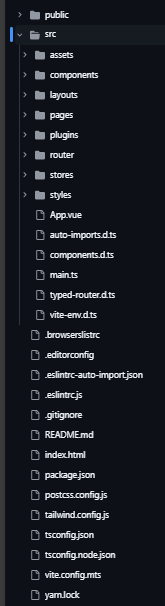
\includegraphics[scale=0.5]{Images/Implement/frontendStructure.png}
    \caption{Cấu trúc Frontend}
\end{figure}

\subsection*{Hệ thống thiết kế (Design System)}

Hệ thống thiết kế được triển khai với mục tiêu cung cấp một giao diện người dùng nhất quán, dễ sử dụng và dễ mở rộng. Hệ thống này bao gồm các thành phần chính sau:

\subsubsection*{Typography}
Typography được xây dựng trên cơ sở font chữ Public Sans, với nhiều kích cỡ và độ đậm khác nhau để phục vụ các nhu cầu hiển thị khác nhau. Font chữ này được chọn vì dễ đọc, phù hợp với các thiết kế hiện đại và hỗ trợ đa ngôn ngữ. Các cấp độ bao gồm:

\begin{itemize}
    \item \textbf{Heading}: Từ Heading 1 (48px, Bold) đến Heading 4 (24px, Semibold).
    \item \textbf{Body Text}: Các cấp độ từ Large đến Small, sử dụng độ đậm từ Regular đến Bold, kích thước từ 10px đến 20px.
\end{itemize}

\begin{figure}[H]
    \centering
    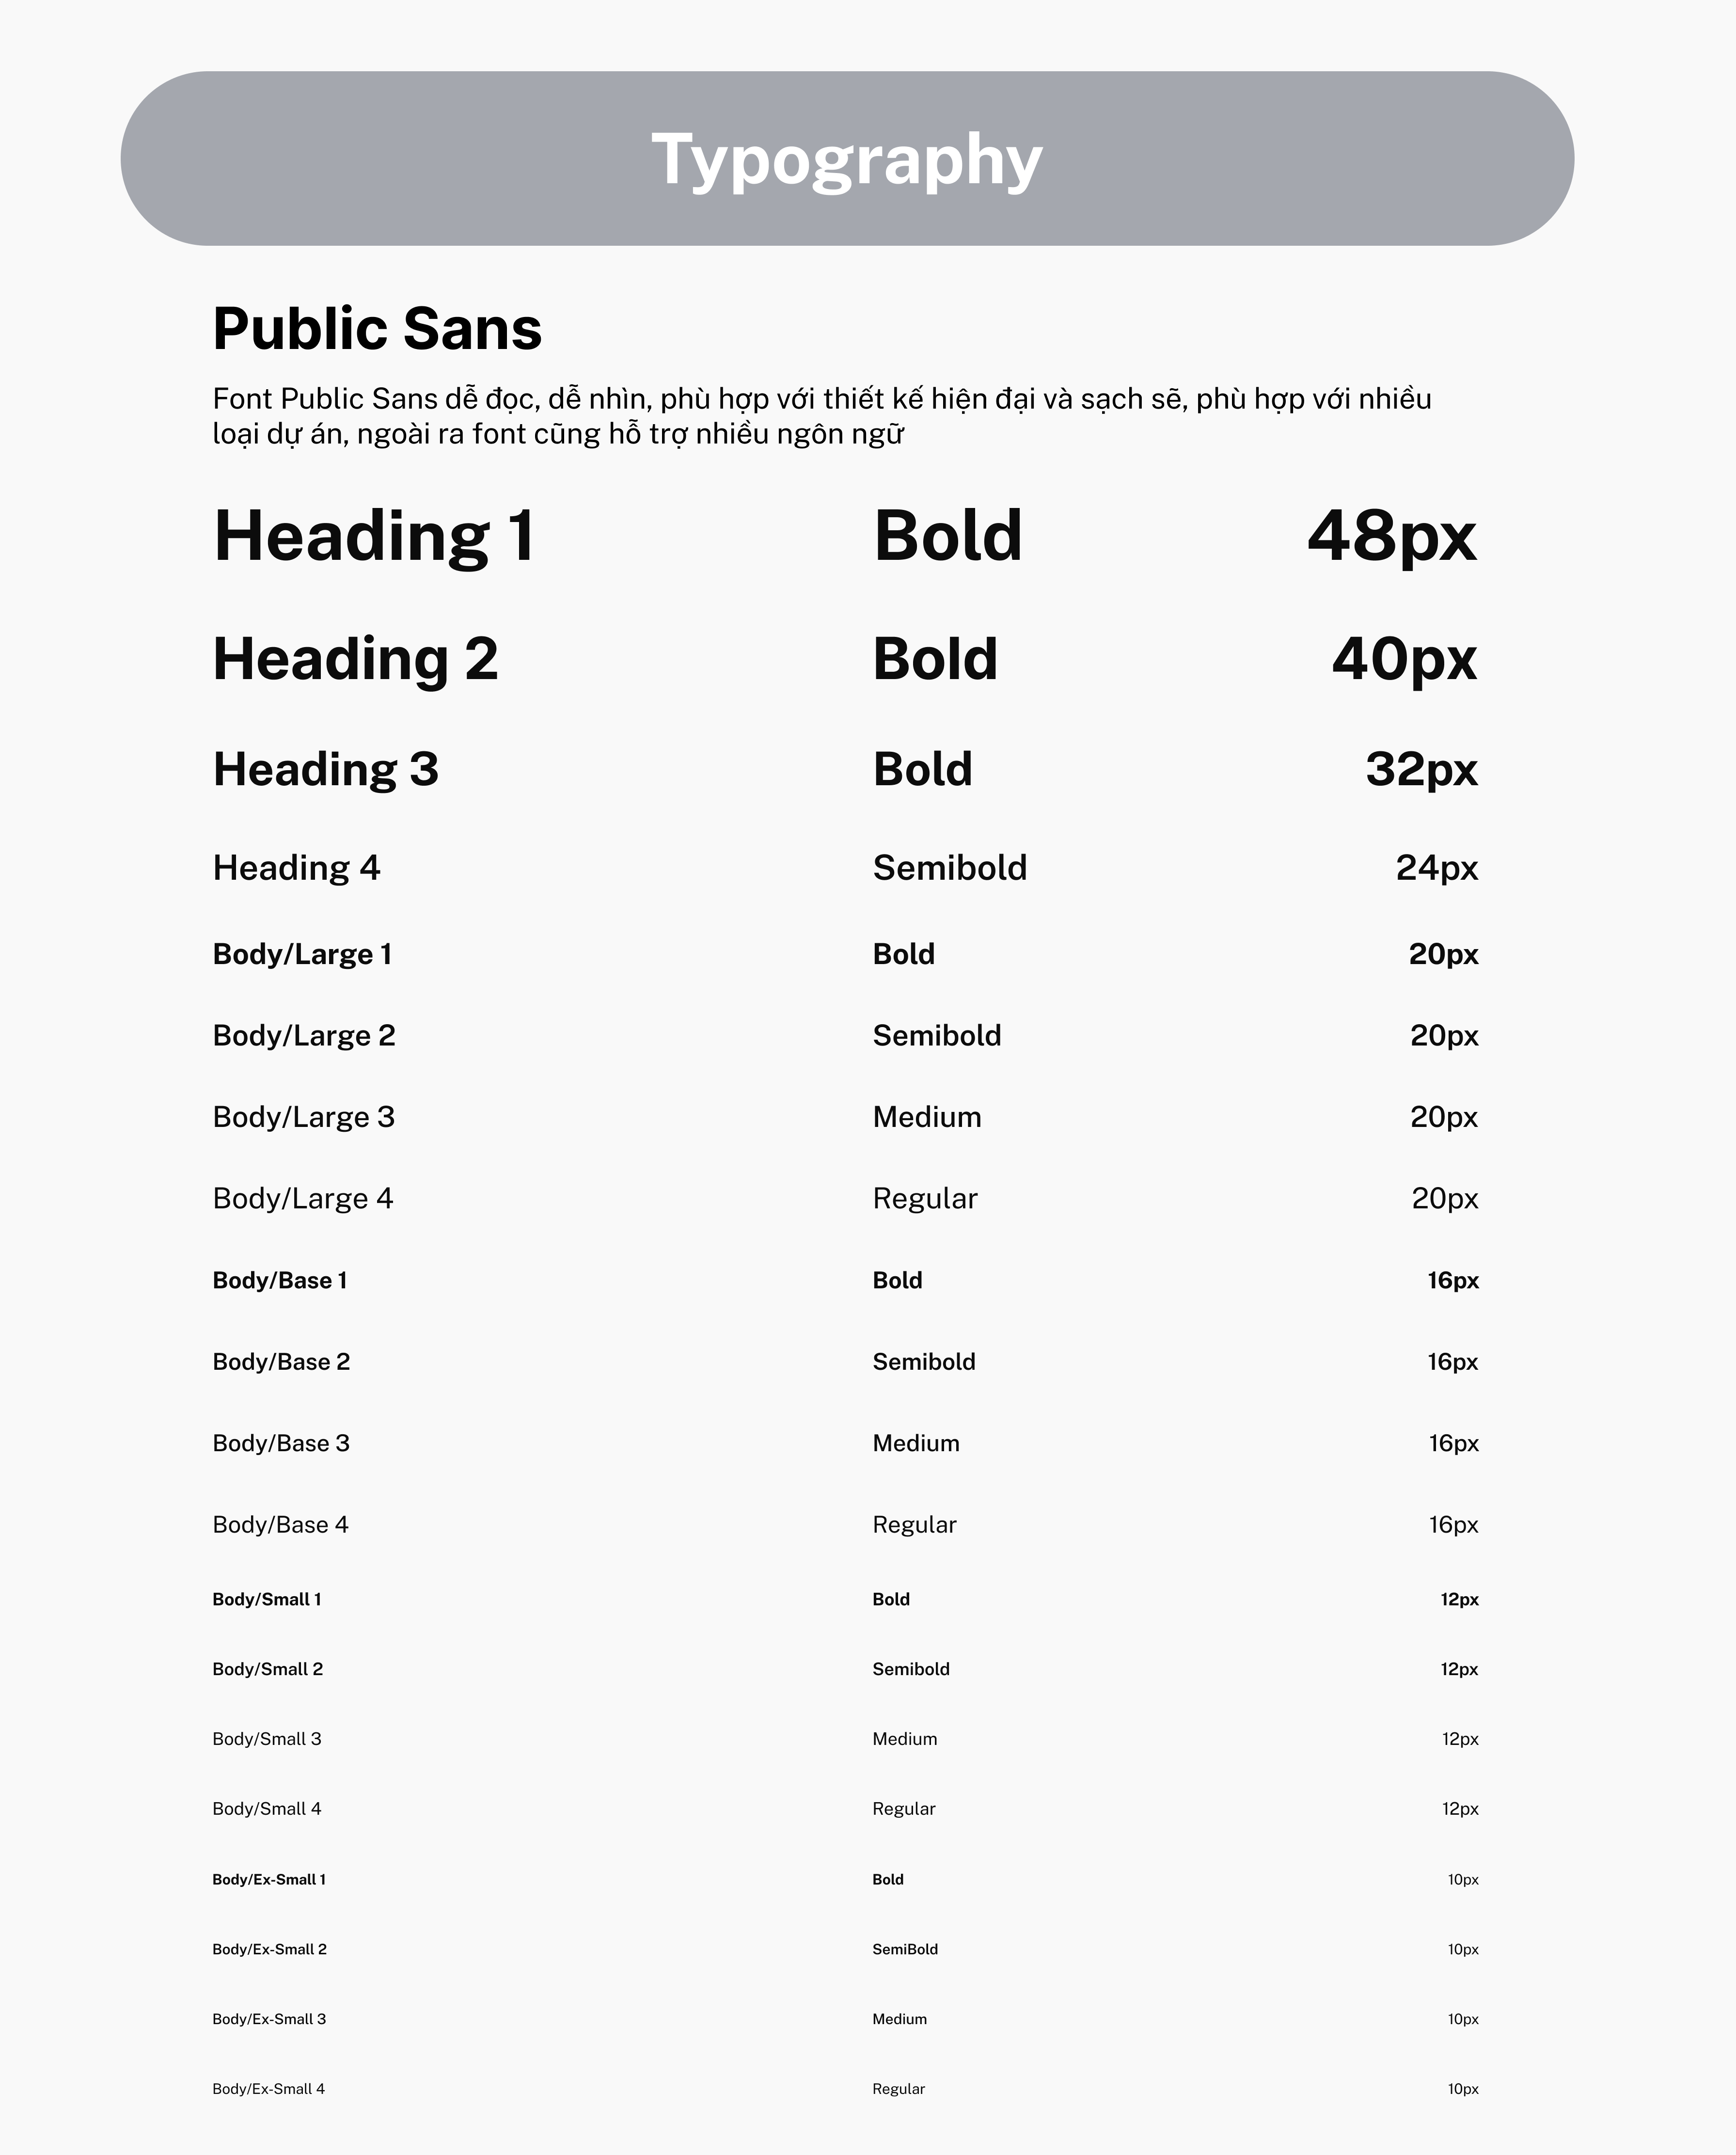
\includegraphics[scale=0.3]{Images/Implement/Typography.png}
    \caption{Hệ thống Typography sử dụng trong ứng dụng}
\end{figure}

\subsubsection*{Bảng màu (Color Palette)}
Bảng màu được thiết kế để mang lại sự nhất quán và dễ nhận biết trong giao diện người dùng. Bảng màu chính bao gồm các màu \textbf{Primary}, \textbf{Secondary}, và các trạng thái như \textbf{Error}, \textbf{Warning}, \textbf{Neutral}, \textbf{Success}. Mỗi màu được chia thành các sắc độ từ nhạt (25, 50) đến đậm (900, 950), nhằm đảm bảo khả năng hiển thị tốt trong các trường hợp sử dụng khác nhau.

\begin{itemize}
    \item \textbf{Primary}: Dùng cho các thành phần chính như nút bấm và tiêu đề.
    \item \textbf{Secondary}: Dùng cho các chi tiết phụ hoặc nhấn mạnh nội dung.
    \item \textbf{Error, Warning, Success}: Dùng để phản hồi trạng thái của hệ thống.
\end{itemize}

\begin{figure}[H]
    \centering
    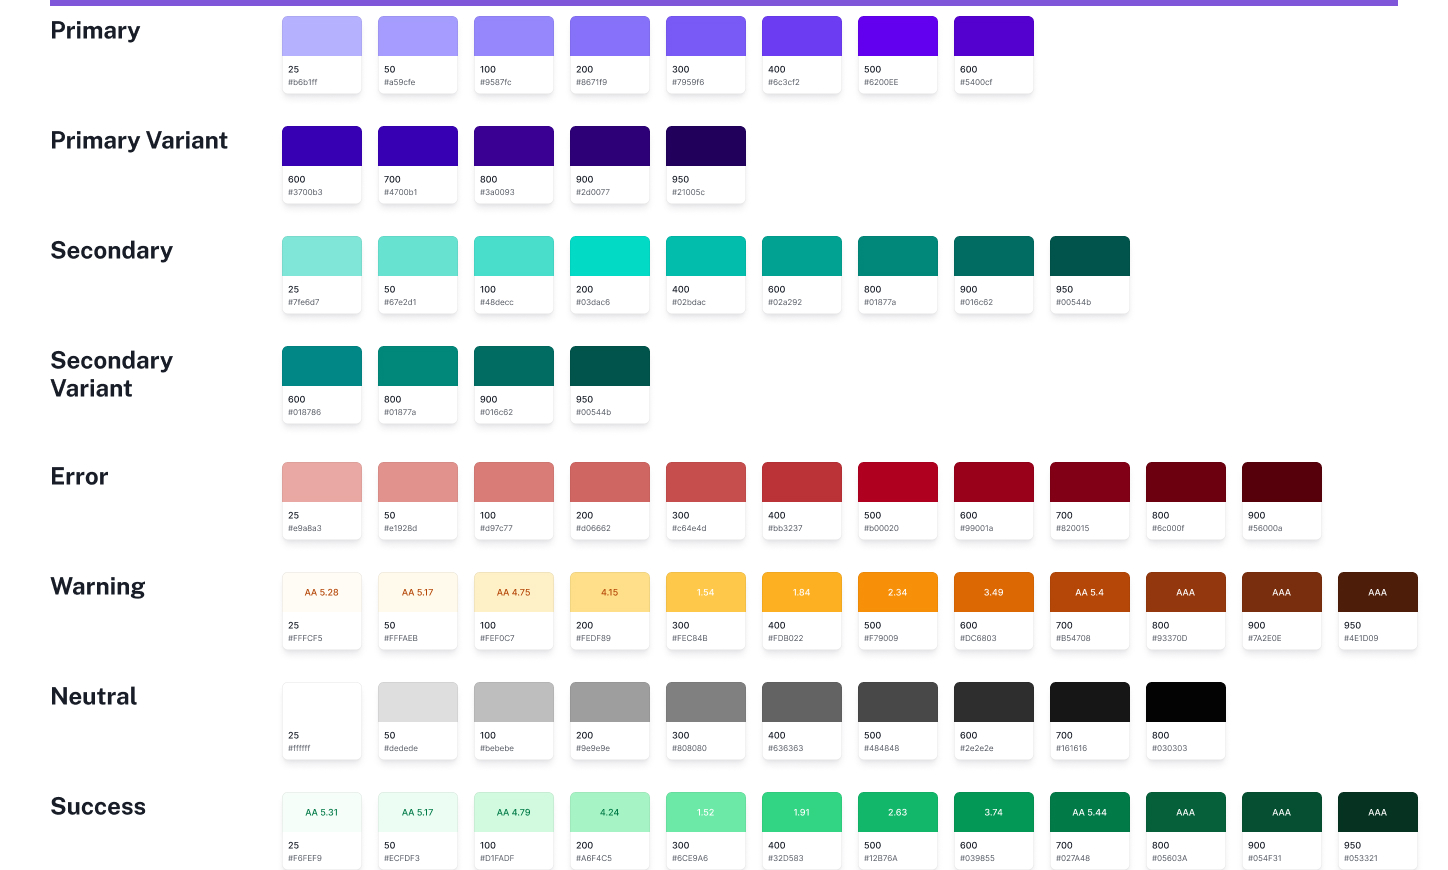
\includegraphics[scale=0.15]{Images/Implement/Colors.jpg}
    \caption{Bảng màu được sử dụng trong ứng dụng}
\end{figure}

Hệ thống này được tích hợp với Tailwind CSS, giúp tự động hóa việc áp dụng các quy tắc thiết kế (design tokens) vào mã nguồn. Điều này làm giảm thiểu lỗi thiết kế, đồng thời đảm bảo giao diện nhất quán trong toàn bộ ứng dụng.


\textbf{Backend}

Backend được phát triển với FastAPI, kết hợp với PostgreSQL để lưu trữ dữ liệu. Kiến trúc hệ thống được tổ chức theo các thành phần chính:
\begin{itemize}
    \item Repository
    \item Provider
    \item Controller
\end{itemize}

Mỗi thành phần đảm nhiệm một vai trò cụ thể, giúp hệ thống trở nên dễ hiểu, có tính tổ chức cao và dễ bảo trì.

\begin{figure}[H]
    \centering
    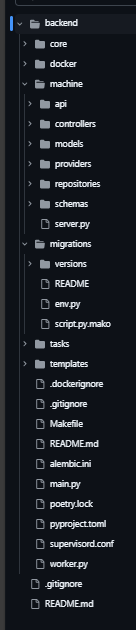
\includegraphics[scale=0.5]{Images/Implement/backendStructure.png}
    \caption{Cấu trúc Backend}
\end{figure}

\section{Kiến trúc Backend}

\textbf{1. Repository} 

Repository chịu trách nhiệm quản lý các thao tác liên quan đến dữ liệu trong hệ thống. Đây là nơi thực hiện các logic liên quan đến việc truy vấn, lưu trữ và cập nhật dữ liệu từ cơ sở dữ liệu PostgreSQL.

Đặc điểm chính:

\begin{itemize}
    \item Tách biệt logic truy xuất dữ liệu khỏi các thành phần khác
    \item Hỗ trợ các thao tác CRUD (Create, Read, Update, Delete)
\end{itemize}

Ví dụ: Repository sẽ xử lý các tác vụ như:

\begin{itemize}
    \item Truy vấn thông tin sinh viên và giảng viên
    \item Cập nhật tiến độ học tập
    \item Xóa thông tin khóa học khi cần thiết
\end{itemize}

\textbf{2. Provider} 

Provider chịu trách nhiệm xử lý các logic nghiệp vụ (business logic). Đây là nơi các phép toán và xử lý phức tạp được thực hiện trước khi trả kết quả cho Controller hoặc người dùng.

Đặc điểm chính:

\begin{itemize}
    \item Không phụ thuộc vào giao diện hoặc nguồn dữ liệu cụ thể
    \item Tập trung vào logic nghiệp vụ và các phép toán quan trọng
\end{itemize}

Ví dụ: Provider sẽ:

\begin{itemize}
    \item Phân tích mục tiêu học tập của sinh viên để đề xuất bài học
    \item Tự động tạo bài học dựa trên nội dung được giảng viên cung cấp
\end{itemize}
 
\textbf{3. Controller} 

Controller là nơi tiếp nhận các yêu cầu từ người dùng thông qua API, sau đó phối hợp với Provider và Repository để thực hiện các chức năng tương ứng.

Đặc điểm chính:

\begin{itemize}
    \item Giao tiếp trực tiếp với frontend thông qua các endpoint API
    \item Chuyển đổi dữ liệu giữa frontend và các thành phần backend
\end{itemize}

Ví dụ: Controller xử lý:

\begin{itemize}
    \item Yêu cầu đăng nhập và xác thực người dùng
    \item Truy xuất danh sách khóa học và chi tiết khóa học
    \item Nhận mục tiêu học tập từ sinh viên và gửi đến Provider để xử lý
\end{itemize}

\section{Quá trình triển khai hệ thống}
\subsection*{Triển khai hệ thống}
\textbf{Frontend:}
Frontend của hệ thống được triển khai trên nền tảng \textbf{Vercel}, mang đến một môi trường ổn định, tối ưu cho việc triển khai các ứng dụng web. Vercel cung cấp khả năng tự động build và deploy mỗi khi có thay đổi trong mã nguồn, giúp quá trình cập nhật trở nên nhanh chóng và mượt mà. Nhờ vào quy trình này, việc triển khai và duy trì hệ thống frontend trở nên đơn giản và hiệu quả.
Vercel không chỉ đảm bảo hiệu suất cao mà còn hỗ trợ các tính năng tối ưu hóa tự động, giúp giảm thời gian tải trang và nâng cao trải nghiệm người dùng. Với khả năng mở rộng linh hoạt, hệ thống có thể dễ dàng đáp ứng với nhu cầu tăng trưởng trong tương lai.
\par \textbf{Link deploy frontend:} \textcolor{blue}{\href{https://codemate-fe-black.vercel.app/}{https://codemate-fe-black.vercel.app/}}

\textbf{Backend:}
Hệ thống sử dụng nền tảng \textbf{Render} để triển khai backend. Render cung cấp một môi trường chạy ổn định, dễ mở rộng và bảo mật cao, giúp tối ưu hóa việc quản lý và triển khai ứng dụng. Với quy trình build và deploy tự động, việc cập nhật hệ thống trở nên mượt mà và hiệu quả, giảm thiểu các vấn đề phát sinh trong quá trình triển khai.
Để triển khai hệ thống, chúng tôi sử dụng công cụ \textbf{Poetry} để quản lý các gói phụ thuộc (dependencies) của Python. Điều này giúp đảm bảo rằng các thư viện và công cụ cần thiết luôn được cài đặt đúng phiên bản, đồng thời giảm thiểu các lỗi liên quan đến môi trường chạy.
Hệ thống được cấu hình để tự động khởi chạy khi có yêu cầu, đảm bảo hiệu suất cao và khả năng mở rộng dễ dàng khi cần thiết. Ngoài ra, Render cũng hỗ trợ giám sát và quản lý môi trường ứng dụng, giúp dễ dàng phát hiện và xử lý các sự cố.
\par \textbf{Link deploy backend:} \textcolor{blue}{\href{https://edumind-5qmn.onrender.com/}{https://edumind-5qmn.onrender.com/}}

\textbf{Quy trình triển khai chi tiết:}
% \begin{figure}[H]
% \centering
% \includegraphics[width=0.85\linewidth]{Images/Implement/DeploymentProcess.png}
% \caption{Quy trình triển khai hệ thống}
% \label{fig}
% \end{figure}
\begin{enumerate}
\item \textbf{Chuẩn bị môi trường phát triển:}
\begin{itemize}
\item Thiết lập môi trường phát triển cục bộ với đầy đủ công cụ cần thiết như Node.js, npm, Python 3.10, và Poetry.
\item Cài đặt các IDE và công cụ phát triển như Visual Studio Code, PyCharm, và Git.
\item Thiết lập hệ thống kiểm soát phiên bản sử dụng GitHub để quản lý mã nguồn và hỗ trợ làm việc nhóm.
\end{itemize}
\item \textbf{Phát triển frontend:}
\begin{itemize}
    \item Sử dụng Vue 3 và Vuetify để xây dựng giao diện người dùng.
    \item Triển khai các component UI theo thiết kế đã được phê duyệt.
    \item Tích hợp các thư viện hỗ trợ như Axios cho việc gọi API, Pinia cho quản lý trạng thái.
    \item Thực hiện tối ưu hóa hiệu suất và khả năng đáp ứng trên các thiết bị khác nhau.
\end{itemize}

\item \textbf{Phát triển backend:}
\begin{itemize}
    \item Xây dựng API sử dụng FastAPI theo kiến trúc Repository-Provider-Controller.
    \item Thiết lập kết nối và tương tác với cơ sở dữ liệu PostgreSQL.
    \item Tích hợp các dịch vụ bên ngoài như Gemini API, Google Authentication.
    \item Phát triển các module xử lý nghiệp vụ chính như quản lý người dùng, quản lý khóa học, đề xuất học tập, và tạo bài tập.
\end{itemize}

\item \textbf{Kiểm thử hệ thống:}
\begin{itemize}
    \item Thực hiện kiểm thử đơn vị cho các thành phần riêng lẻ.
    \item Kiểm thử tích hợp để đảm bảo các thành phần phối hợp tốt với nhau.
    \item Kiểm thử chức năng để xác nhận các tính năng hoạt động đúng theo yêu cầu.
    \item Kiểm thử hiệu suất để đánh giá khả năng đáp ứng và xử lý tải của hệ thống.
\end{itemize}

\item \textbf{Triển khai trên môi trường cloud:}
\begin{itemize}
    \item Thiết lập môi trường cloud trên Vercel cho frontend và Render cho backend.
    \item Cấu hình các biến môi trường và thiết lập bảo mật.
    \item Thiết lập quy trình CI/CD để tự động hóa việc build và deploy khi có thay đổi trong mã nguồn.
    \item Cài đặt và cấu hình cơ sở dữ liệu PostgreSQL trên nền tảng đám mây.
\end{itemize}

% \item \textbf{Giám sát và bảo trì:}
% \begin{itemize}
%     \item Thiết lập hệ thống giám sát để theo dõi hiệu suất và phát hiện sự cố.
%     \item Triển khai quy trình cập nhật và bảo trì định kỳ.
%     \item Phân tích dữ liệu sử dụng để cải thiện trải nghiệm người dùng và tối ưu hóa hiệu suất.
%     \item Xử lý các vấn đề và cải tiến hệ thống dựa trên phản hồi từ người dùng.
% \end{itemize}
\end{enumerate}
\textbf{Các công nghệ được sử dụng trong triển khai:}
\begin{table}[H]
\centering
\begin{tabularx}{\textwidth}{|l|X|}
\hline
\textbf{Lĩnh vực} & \textbf{Công nghệ} \\ \hline
Frontend & Vue 3, Vuetify, Tailwind CSS, Pinia, Axios, Jest \\ \hline
Backend & FastAPI, SQLAlchemy, Pydantic, LangChain, Alembic \\ \hline
Cơ sở dữ liệu & PostgreSQL, Redis (cache) \\ \hline
AI & OpenAI API (GPT-4o), Google Gemini API \\ \hline
Triển khai & Vercel (Frontend), Render (Backend), GitHub Actions (CI/CD) \\ \hline
% Giám sát & Sentry, Prometheus, Grafana \\ \hline
\end{tabularx}
\caption{Các công nghệ sử dụng trong quá trình triển khai}
\label{table}
\end{table}
% \textbf{Kết quả triển khai:}
% Sau khi hoàn thành quá trình triển khai, hệ thống đã được đưa vào vận hành thử nghiệm với một nhóm người dùng ban đầu. Kết quả thu được rất khả quan, với thời gian phản hồi nhanh và trải nghiệm người dùng mượt mà. Hệ thống đã xử lý được hơn 500 yêu cầu đồng thời trong các đợt kiểm tra tải, đảm bảo khả năng phục vụ số lượng lớn người dùng trong tương lai.
% Các tính năng chính như đề xuất lộ trình học tập, tạo bài tập tự động, và gia sư AI đều hoạt động tốt trong môi trường sản xuất, với thời gian phản hồi trung bình cho các yêu cầu AI dưới 5 giây, đáp ứng yêu cầu về hiệu suất đề ra.
% \begin{figure}[H]
% \centering
% \includegraphics[width=0.85\linewidth]{Images/Implement/SystemPerformance.png}
% \caption{Biểu đồ hiệu suất hệ thống sau khi triển khai}
% \label{fig}
% \end{figure}
% Quá trình triển khai hệ thống đã diễn ra suôn sẻ, với các vấn đề phát sinh được xử lý kịp thời. Hệ thống hiện đang hoạt động ổn định và sẵn sàng cho việc mở rộng quy mô trong tương lai.
% \section{Các chức năng đã được thực hiện}

% Dưới đây là các chức năng đã được thực hiện trong hệ thống học tập trực tuyến thông minh. Các chức năng này được phân chia theo từng module và vai trò của người dùng trong hệ thống.

% \subsection{Quản lý tài khoản (Thành viên đảm nhiệm: Phạm Thi)}
% Module này cung cấp các chức năng liên quan đến đăng nhập, xác thực và quản lý thông tin cá nhân của người dùng.
% \begin{itemize}[label=--]
%     \item Đăng nhập vào hệ thống bằng email/mật khẩu hoặc tài khoản Google (Role: Sinh viên, Giảng viên, Quản trị viên).
%     \item Làm mới token xác thực khi phiên đăng nhập hết hạn (Role: Sinh viên, Giảng viên, Quản trị viên).
%     \item Xác minh email và gửi lại mã xác minh nếu cần (Role: Sinh viên, Giảng viên, Quản trị viên).
%     \item Đặt lại mật khẩu khi quên mật khẩu (Role: Sinh viên, Giảng viên, Quản trị viên).
%     \item Cập nhật thông tin cá nhân (tên, ngày sinh, ảnh đại diện) (Role: Sinh viên, Giảng viên, Quản trị viên).
%     \item Xem thông tin hồ sơ cá nhân (ID, tên, email, MSSV/MSCB, ngày sinh, vai trò) (Role: Sinh viên, Giảng viên, Quản trị viên).
% \end{itemize}

% \begin{figure}[H]
%     \centering
%     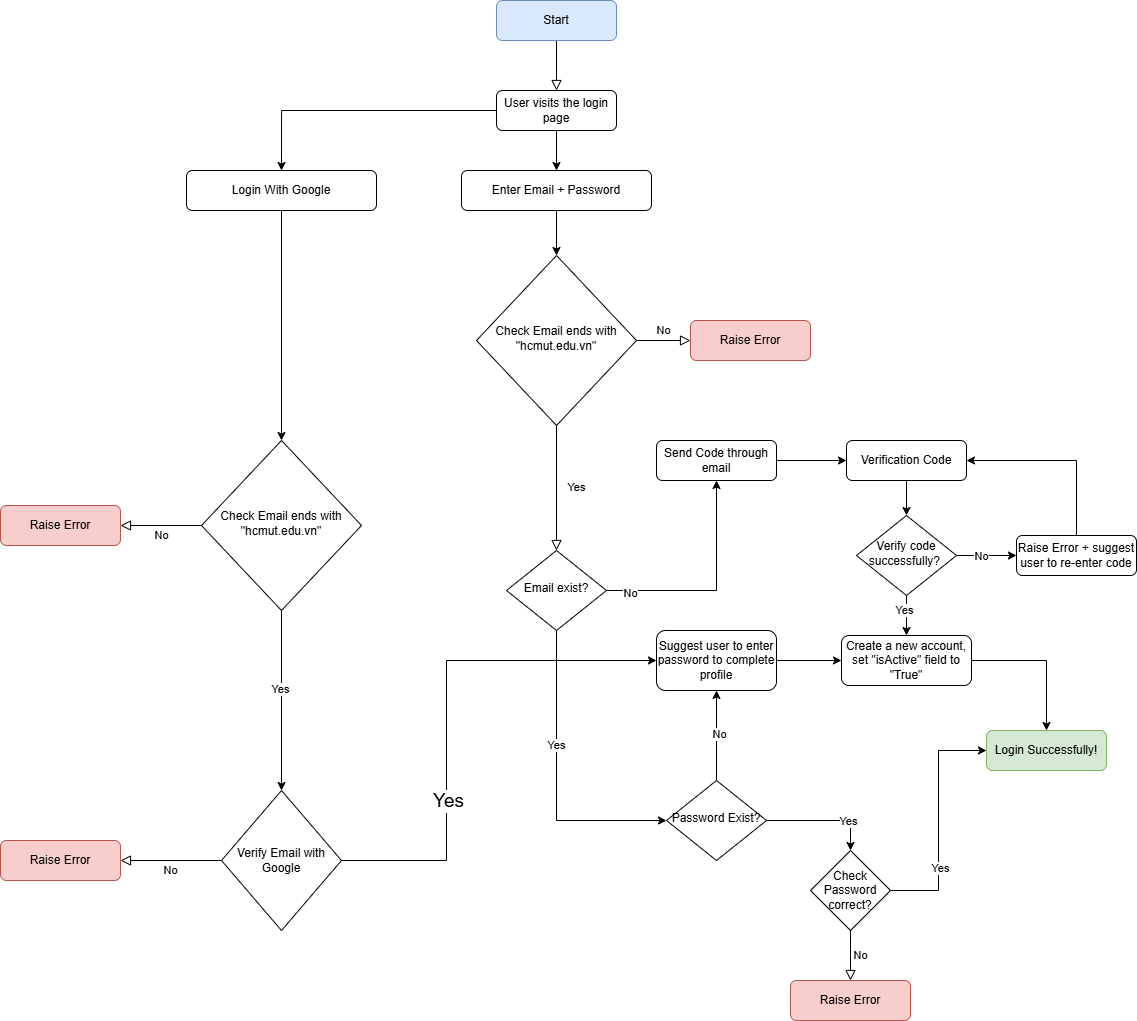
\includegraphics[width=0.9\linewidth]{images/Quan_ly_tai_khoan/authenFlow.drawio.png}
%     \caption{Flow Định danh tài khoản}
%     \label{fig:enter-label}
% \end{figure}

% \subsection{Quản lý khóa học (Thành viên đảm nhiệm: Phạm Thi/Tuấn Anh)}
% Module này hỗ trợ quản lý thông tin khóa học, bao gồm tạo, xem, cập nhật và xóa dữ liệu liên quan.
% \begin{itemize}[label=--]
%     \item Xem danh sách khóa học (đã đăng ký hoặc đang phụ trách, hỗ trợ phân trang và tìm kiếm) (Role: Sinh viên, Giảng viên).
%     \item Xem chi tiết khóa học (số lượng sinh viên, bài học, bài tập, tài liệu, tiến độ học tập) (Role: Sinh viên, Giảng viên).
%     \item Xem thông tin Giảng viên của khóa học (Role: Sinh viên).
%     \item Cập nhật mục tiêu học tập và ảnh khóa học (Role: Giảng viên).
%     \item Tạo khóa học mới (đơn lẻ hoặc nhiều khóa) (Role: Quản trị viên).
%     \item Cập nhật thông tin khóa học (tên, tín chỉ, học kỳ) (Role: Quản trị viên).
%     \item Xóa khóa học cùng dữ liệu liên quan (Role: Quản trị viên).
%     \item Xem danh sách khóa học có sẵn của HCMUT (Role: Quản trị viên).
%     \item Xem khóa học truy cập gần đây nhất qua dashboard (Role: Sinh viên).
% \end{itemize}

% \subsection{Quản lý bài học (Thành viên đảm nhiệm: Phạm Thi/Tuấn Anh)}
% Module này cho phép tạo, chỉnh sửa và quản lý bài học trong khóa học.
% \begin{itemize}[label=--]
%     \item Xem danh sách bài học trong khóa học (Role: Sinh viên).
%     \item Tạo bài học mới (Role: Giảng viên).
%     \item Cập nhật bài học (tiêu đề, mô tả, mục tiêu học tập) (Role: Giảng viên).
%     \item Xóa bài học cùng tài liệu liên quan (Role: Giảng viên).
%     \item Thêm tài liệu vào bài học (Role: Giảng viên).
%     \item Xem chi tiết bài học và danh sách tài liệu liên quan (Role: Giảng viên).
% \end{itemize}

% \subsection{Quản lý bài tập (Thành viên đảm nhiệm: Tuấn Anh)}
% Module này hỗ trợ quản lý bài tập dạng quiz và lập trình, bao gồm tạo, xem và nộp bài.
% \begin{itemize}[label=--]
%     \item Xem danh sách bài tập trong khóa học (chỉ bài tập đã mở) (Role: Sinh viên).
%     \item Xem chi tiết bài tập dạng quiz hoặc lập trình (câu hỏi, yêu cầu, test cases) (Role: Sinh viên, Giảng viên).
%     \item Tạo bài tập dạng quiz hoặc lập trình (Role: Giảng viên).
%     \item Cập nhật thông tin bài tập dạng quiz hoặc lập trình (Role: Giảng viên).
%     \item Xóa bài tập dạng quiz hoặc lập trình (Role: Giảng viên).
%     \item Gửi câu hỏi tới trợ lý lập trình và xem lịch sử hội thoại (Role: Sinh viên).
%     \item Nộp bài quiz và xóa câu trả lời để làm lại (Role: Sinh viên).
%     \item Xem danh sách sự kiện bài tập sắp tới qua lịch học (Role: Sinh viên, Giảng viên).
% \end{itemize}

% \subsection{Quản lý lộ trình học tập (Thành viên đảm nhiệm: Phạm Thi/Tuấn Anh)}
% Module này cung cấp các chức năng liên quan đến lộ trình học tập cá nhân hóa và bài học đề xuất.
% \begin{itemize}[label=--]
%     \item Xem lộ trình học tập cá nhân hóa và danh sách bài học đề xuất (Role: Sinh viên).
%     \item Xóa lộ trình học tập cá nhân (Role: Sinh viên).
%     \item Xem chi tiết bài học đề xuất (tiêu đề, mục tiêu, nội dung, tiến độ) (Role: Sinh viên).
%     \item Đánh dấu hoặc bỏ đánh dấu bài học đề xuất (Role: Sinh viên).
%     \item Yêu cầu tạo lộ trình học tập dựa trên mục tiêu và khóa học (Role: Sinh viên).
%     \item Tái tạo nội dung bài học dựa trên vấn đề đã xác định (Role: Sinh viên).
%     \item Nhận gợi ý mục tiêu học tập từ hệ thống (Role: Sinh viên).
%     \item Xem tài liệu của module trong lộ trình học tập (Role: Sinh viên).
%     \item Tạo bài quiz dựa trên nội dung module (Role: Sinh viên).
% \end{itemize}

% \subsection{Theo dõi tiến độ học tập (Thành viên đảm nhiệm: Phạm Thi/Tuấn Anh)}
% Module này hỗ trợ theo dõi và đánh giá tiến độ học tập của sinh viên.
% \begin{itemize}[label=--]
%     \item Nhận đánh giá tiến độ học tập theo chuẩn Rubric (Role: Sinh viên).
%     \item Cập nhật thời gian học cho bài học đề xuất (Role: Sinh viên).
%     \item Xem phân tích tiến độ học tập trong khóa học hoặc bài học cụ thể (Role: Sinh viên).
%     \item Xem điểm số của sinh viên trong khóa học (tên, email, MSSV, điểm trung bình) (Role: Giảng viên).
%     \item Xem điểm chi tiết của một bài tập cụ thể (Role: Giảng viên).
% \end{itemize}

% \subsection{Quản lý phản hồi (Thành viên đảm nhiệm: Phạm Thi)}
% Module này cho phép gửi, xem và quản lý phản hồi trong hệ thống.
% \begin{itemize}[label=--]
%     \item Gửi phản hồi về hệ thống hoặc khóa học (tiêu đề, mô tả, đánh giá) (Role: Sinh viên, Giảng viên).
%     \item Xem danh sách phản hồi (lọc theo tháng, năm, trạng thái, khóa học) (Role: Giảng viên, Quản trị viên).
%     \item Cập nhật trạng thái phản hồi (pending, in\_progress, resolved) (Role: Quản trị viên).
%     \item Xóa phản hồi khỏi hệ thống (Role: Quản trị viên).
% \end{itemize}

% \subsection{Quản lý người dùng (Thành viên đảm nhiệm: Phạm Thi)}
% Module này cung cấp các chức năng quản lý thông tin và trạng thái người dùng trong hệ thống.
% \begin{itemize}[label=--]
%     \item Tạo người dùng mới (sinh viên, Giảng viên, quản trị viên) (Role: Quản trị viên).
%     \item Đếm số lượng người dùng (tổng hoặc theo vai trò) (Role: Quản trị viên).
%     \item Xem danh sách tất cả người dùng (lọc theo vai trò, trạng thái, tìm kiếm) (Role: Quản trị viên).
%     \item Xem thông tin chi tiết của một người dùng cụ thể (Role: Quản trị viên).
%     \item Cập nhật trạng thái người dùng (bật/tắt) (Role: Quản trị viên).
% \end{itemize}

% \subsection{Quản lý nhật ký đăng nhập (Thành viên đảm nhiệm: Phạm Thi)}
% Module này hỗ trợ theo dõi và ghi nhận hoạt động đăng nhập của người dùng.
% \begin{itemize}[label=--]
%     \item Xem danh sách nhật ký đăng nhập (ID người dùng, vai trò, thời gian) (Role: Quản trị viên).
%     \item Tạo bản ghi nhật ký đăng nhập mới (Role: Quản trị viên).
% \end{itemize}

% \subsection{Quản lý dashboard (Thành viên đảm nhiệm: Phạm Thi)}
% Module này cung cấp tổng quan hoạt động cho người dùng qua giao diện dashboard.
% \begin{itemize}[label=--]
%     \item Xem tổng quan hoạt động giảng dạy (số lượng khóa học, bài học, sinh viên, bài tập) (Role: Giảng viên).
%     \item Xem và thêm các hoạt động gần đây (tối đa 5 hoạt động) (Role: Sinh viên).
% \end{itemize}

% \subsection{Code Assistant (Thành viên đảm nhiệm: Phương Nam)}
% Module này hỗ trợ sinh viên trong việc lập trình và giải quyết các vấn đề liên quan đến mã nguồn.
% \begin{itemize}[label=--]
%     \item Gợi ý mã nguồn dựa trên yêu cầu của sinh viên (Role: Sinh viên).
%     \item Tạo bài kiểm tra lập trình dựa trên nội dung module (Role: Sinh viên).
%     \item Hỗ trợ kiểm tra mã nguồn và đưa ra các gợi ý sửa lỗi (Role: Sinh viên).
%     \item Hướng dẫn sinh viên trong việc giải quyết các vấn đề lập trình (Role: Sinh viên).
%     \item Chatbot hỗ trợ sinh viên trong việc lập trình và giải quyết các vấn đề liên quan đến mã nguồn (Role: Sinh viên).
% \end{itemize}
% \section{Giới thiệu chi tiết về các chức năng chính của hệ thống}
% Hệ thống học tập thông minh được thiết kế để hỗ trợ học sinh trong việc lập kế hoạch học tập và đánh giá tiến độ một cách hiệu quả. Với sự tích hợp của AI, hệ thống có khả năng phân tích dữ liệu học tập, tạo lộ trình cá nhân hóa và đưa ra các đánh giá chi tiết. Mục nội dung này sẽ tập trung vào các chức năng chính như sinh ra lộ trình học tập, đề xuất mục tiêu học tập, đánh giá kết quả học tập, tạo bài kiểm tra, và các tính năng bổ sung khác. \par 

% Sau đây là các nguyên tắc cơ bản trong việc thiết lập mục tiêu học tập và phương pháp đánh giá mà hệ thống áp dụng:

% \subsection{Nguyên tắc SMART trong việc thiết lập mục tiêu}
% Nguyên tắc SMART là một khung tiêu chuẩn được áp dụng rộng rãi trong việc thiết lập mục tiêu hiệu quả. Trong hệ thống của chúng tôi, mỗi mục tiêu học tập được đề xuất đều tuân theo năm tiêu chí của nguyên tắc SMART:

% \begin{itemize}
%     \item \textbf{Specific (Cụ thể)}: Mục tiêu phải rõ ràng và cụ thể, không mơ hồ. Ví dụ: ``Hiểu và áp dụng được các thuật toán sắp xếp'' thay vì ``Học về thuật toán''.
    
%     \item \textbf{Measurable (Đo lường được)}: Mục tiêu phải có thể đo lường được để đánh giá tiến độ. Ví dụ: ``Đạt điểm 8/10 trong bài kiểm tra về cấu trúc dữ liệu'' hoặc ``Hoàn thành 5 bài tập lập trình về đệ quy''.
    
%     \item \textbf{Achievable (Khả thi)}: Mục tiêu phải thực tế và có thể đạt được với các nguồn lực và thời gian hiện có. Mục tiêu quá tham vọng có thể dẫn đến nản chí.
    
%     \item \textbf{Relevant (Liên quan)}: Mục tiêu phải phù hợp với nội dung khóa học và kết quả học tập mong đợi. Ví dụ, đặt mục tiêu học sâu về machine learning sẽ không phù hợp cho một khóa học cơ bản về Python.
    
%     \item \textbf{Time-bound (Giới hạn thời gian)}: Mục tiêu phải có thời hạn cụ thể để tạo động lực và tính cấp bách. Ví dụ: ``Hoàn thành trước kỳ thi giữa kỳ'' hoặc ``Trong vòng 3 tuần''.
% \end{itemize}

% Trong API \texttt{/generate-student-goals}, AI sẽ tạo ra các mục tiêu học tập tuân thủ nguyên tắc SMART cho ba cấp độ học tập khác nhau: Struggling (khó khăn), Average (trung bình), và Advanced (nâng cao). Mỗi mục tiêu đều được giới hạn dưới 200 ký tự để đảm bảo tính súc tích và dễ nhớ.

% \subsection{Phương pháp Rubric-Based Assessment}
% Rubric-Based Assessment (Đánh giá dựa trên Rubric) là phương pháp đánh giá sử dụng các tiêu chí cụ thể và mức độ đạt được cho mỗi tiêu chí. Phương pháp này mang lại nhiều lợi ích:

% \begin{itemize}
%     \item \textbf{Tính khách quan}: Đánh giá dựa trên các tiêu chí rõ ràng, giảm thiểu tính chủ quan.
%     \item \textbf{Tính nhất quán}: Đảm bảo các học sinh được đánh giá theo cùng một tiêu chuẩn.
%     \item \textbf{Tính minh bạch}: Học sinh hiểu rõ họ được đánh giá như thế nào và cần cải thiện điều gì.
%     \item \textbf{Phản hồi có cấu trúc}: Cung cấp phản hồi chi tiết theo từng tiêu chí.
% \end{itemize}

% Trong hệ thống của chúng tôi, Rubric được áp dụng để đánh giá học sinh theo ba tiêu chí chính:
% \begin{enumerate}
%     \item \textbf{Kiến thức lý thuyết (Theoretical Knowledge)}: Đánh giá mức độ hiểu biết về lý thuyết dựa trên tiến độ trong các bài học liên quan đến khái niệm lý thuyết.
    
%     \item \textbf{Kỹ năng thực hành (Coding Skills)}: Đánh giá kỹ năng lập trình dựa trên việc hoàn thành các bài tập mã hóa. Nếu khóa học không bao gồm lập trình, tiêu chí này sẽ được thay thế bằng một kỹ năng thực hành khác phù hợp.
    
%     \item \textbf{Nỗ lực (Effort)}: Đánh giá sự cố gắng dựa trên thời gian học tập (time\_spent), số lượng bài học đã bắt đầu (status), và tiến độ tổng thể.
% \end{enumerate}

% Mỗi tiêu chí được đánh giá theo bốn mức độ: Excellent (Xuất sắc), Good (Tốt), Average (Trung bình), và Poor (Kém), với các miêu tả cụ thể cho mỗi mức độ.

% \subsection{Phương pháp đánh giá STAR}
% STAR là một phương pháp đánh giá cấu trúc được sử dụng rộng rãi trong giáo dục và phát triển nghề nghiệp. Trong hệ thống của chúng tôi, phương pháp STAR được áp dụng để đánh giá tiến độ học tập của học sinh một cách toàn diện. STAR bao gồm bốn thành phần:

% \begin{itemize}
%     \item \textbf{Situation (Tình huống)}: Mô tả bối cảnh học tập của học sinh, bao gồm tên, khóa học, và mối liên hệ với mục tiêu học tập.
    
%     \item \textbf{Task (Nhiệm vụ)}: Nêu rõ mục tiêu học tập của học sinh, nhấn mạnh tầm quan trọng của việc đạt được mục tiêu trước thời hạn (ví dụ: trước kỳ thi giữa kỳ).
    
%     \item \textbf{Action (Hành động)}: Liệt kê chi tiết các hành động học sinh đã thực hiện cho mỗi tiêu chí đánh giá (Kiến thức lý thuyết, Kỹ năng thực hành, Nỗ lực), dựa trên dữ liệu bài học (progress, time\_spent, objectives).
    
%     \item \textbf{Result (Kết quả)}: Đánh giá tiến độ tổng thể so với mục tiêu, phân tích theo từng tiêu chí, với nhận xét rõ ràng (on track/needs effort/at risk) và tham chiếu đến ngày hiện tại.
% \end{itemize}

% API \texttt{/student/\{courseId\}/assessment} sử dụng phương pháp STAR kết hợp với Rubric để tạo ra báo cáo đánh giá toàn diện cho học sinh, giúp họ hiểu rõ tiến độ học tập và những điểm cần cải thiện.

\section{Sinh ra lộ trình học tập}
Chức năng này chịu trách nhiệm tạo ra một lộ trình học tập cá nhân hóa dựa trên mục tiêu học tập của học sinh, nội dung khóa học và thời gian khả dụng. Quá trình được thực hiện qua ba giai đoạn chính:

\begin{enumerate}
    \item \textbf{Phân tích mục tiêu và thời gian}: Hàm \texttt{analyze\_goal\_and\_timeline} kiểm tra tính hợp lệ của mục tiêu (ví dụ: độ dài, tính liên quan) và xác định thời gian khả thi dựa trên ngày bắt đầu và kết thúc khóa học. Ví dụ mã nguồn:
    \begin{lstlisting}[language=Python]
async def analyze_goal_and_timeline(goal: str, course_start_date: datetime, ...):
    if len(goal) < 10:
        raise ApplicationException(message="Goal is too short...")
    prompt = f"..."
    chunking_manager = ChunkingManager(
        provider="gemini",
        gemini_model_name="gemini-2.0-flash-lite",
        max_tokens_per_chunk=15000,
        temperature=0.7,
        max_output_tokens=8000
    )
    response = chunking_manager.call_llm_api(prompt, "You are an expert in goal validation and timeline analysis.")
    \end{lstlisting}

    \item \textbf{Lựa chọn bài học liên quan}: Hàm \texttt{select\_relevant\_lessons} lọc các bài học phù hợp với mục tiêu, sắp xếp theo thứ tự logic và điều chỉnh theo thời gian. AI được sử dụng để ưu tiên các bài học nền tảng nếu thời gian ngắn.

    \item \textbf{Tạo lộ trình chi tiết}: Hàm \texttt{generate\_detailed\_learning\_path} xây dựng lộ trình đầy đủ, bao gồm các bài học được đề xuất và phân bổ thời gian cụ thể. Kết quả được lưu vào cơ sở dữ liệu qua endpoint \texttt{/generate-learning-path}.
\end{enumerate}

Kết quả là một JSON chứa thông tin chi tiết về lộ trình, ví dụ:
\begin{lstlisting}[language=JSON]
{
    "learning_path_start_date": "2025-04-06",
    "learning_path_end_date": "2025-05-20",
    "learning_path_objective": "Achieve goal...",
    "recommend_lessons": [
        {
            "lesson_id": "123",
            "recommended_content": "What to focus on in this lesson...",
            "explain": "Why this lesson supports the goal...",
            "order": 1,
            "number_of_modules": 2
        }
    ],
    "modules": [
        {
            "title": "Module Title",
            "objectives": ["Objective 1", "Objective 2"],
            "reading_material": {...}
        }
    ]
}
\end{lstlisting}

Kết quả giao diện một lộ trình học tập cơ bản, ví dụ:
\begin{figure}[H]
    \centering
    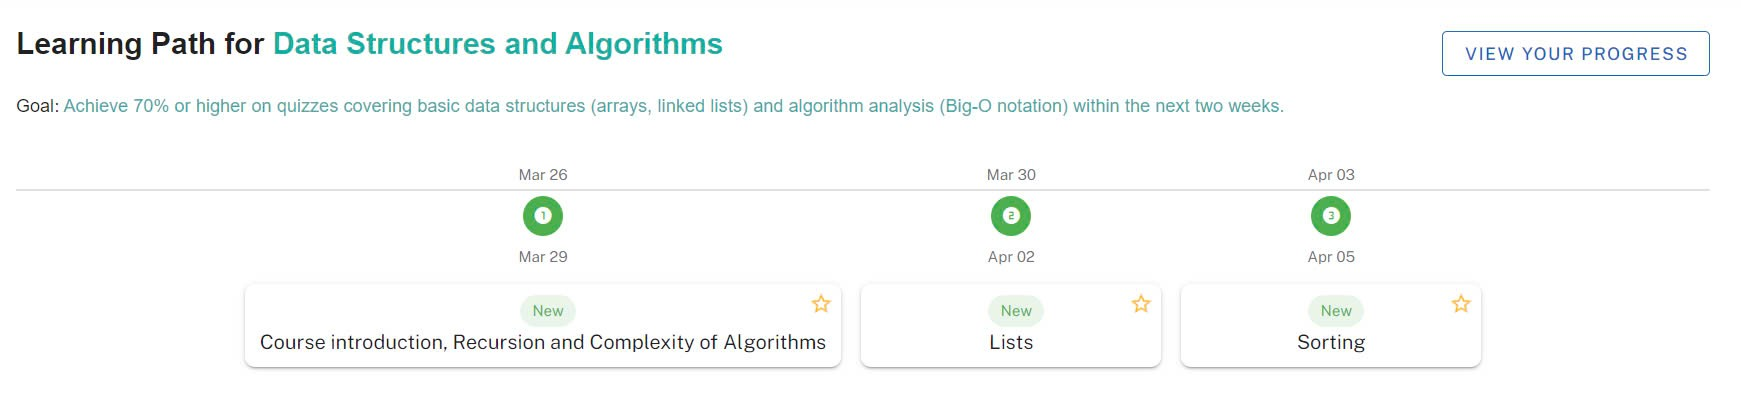
\includegraphics[width=0.8\textwidth]{Images/UI_LLM/Learning_Path.png}
    \caption{Lộ trình học tập cá nhân hóa dựa trên mục tiêu sinh viên}
\end{figure}
\begin{figure}[H]
    \centering
    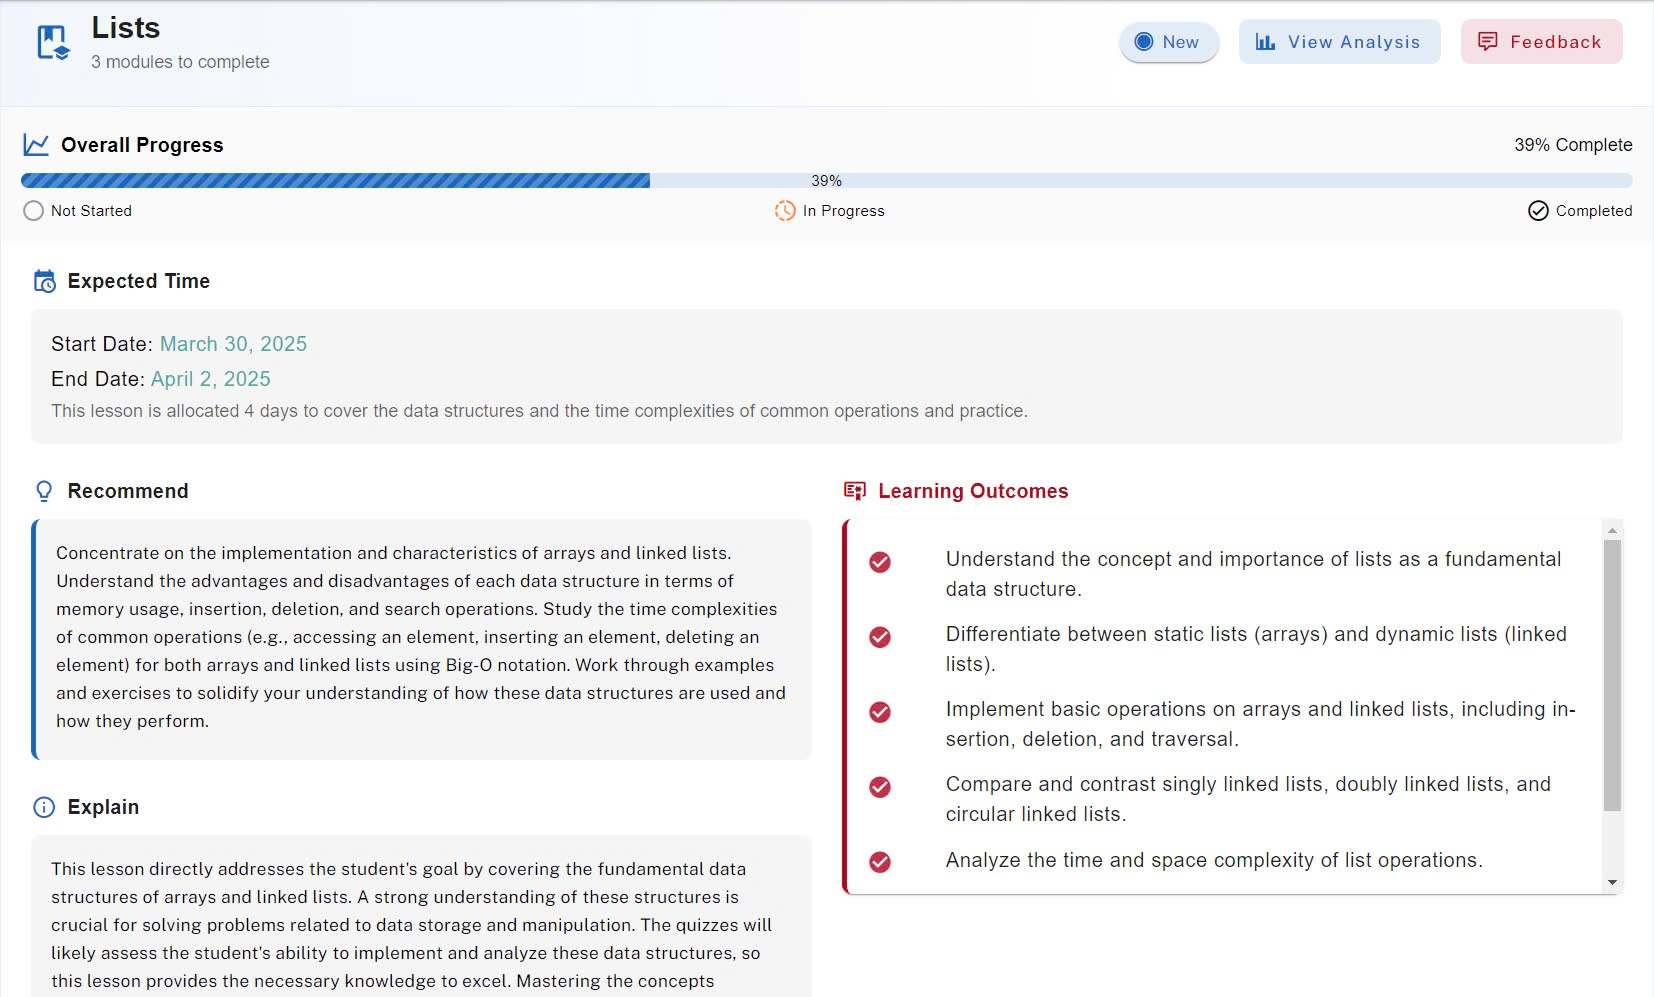
\includegraphics[width=0.8\textwidth]{Images/UI_LLM/Lesson_detail.png}
    \caption{Chi tiết một bài học trong lộ trình}
\end{figure}
\section{Đề xuất mục tiêu học tập}
Đây là tính năng mới được thêm vào để giúp học sinh xác định mục tiêu học tập phù hợp, sử dụng endpoint \texttt{/generate-student-goals/\{course\_id\}}. Các bước thực hiện:

\begin{itemize}
    \item \textbf{Thu thập thông tin khóa học}: Hệ thống lấy dữ liệu về tên khóa học, mục tiêu học tập, và tổng quan các bài học.
    \item \textbf{Sinh mục tiêu theo trình độ}: AI tạo ra các mục tiêu học tập phù hợp cho ba cấp độ khác nhau: Struggling (khó khăn), Average (trung bình), và Advanced (nâng cao), mỗi cấp độ có 2-3 mục tiêu cụ thể.
    \item \textbf{Đảm bảo chất lượng mục tiêu}: Mỗi mục tiêu đều tuân theo nguyên tắc SMART (Specific, Measurable, Achievable, Relevant, Time-bound) và không vượt quá 200 ký tự.
\end{itemize}

Kết quả là một JSON chứa các mục tiêu học tập được đề xuất, ví dụ:
\begin{lstlisting}[language=JSON]
{
    "suggested_goals": [
        {
            "proficiency_level": "Struggling",
            "goal": "Master basic Python syntax and write simple programs with 70% accuracy by midterm",
            "explanation": "This goal focuses on building fundamental programming skills...",
            "key_lessons": ["Introduction to Python", "Basic Data Types"]
        },
        {
            "proficiency_level": "Average",
            "goal": "Implement and optimize sorting algorithms with 80% efficiency by midterm",
            "explanation": "This goal challenges the student to apply theoretical concepts...",
            "key_lessons": ["Algorithm Complexity", "Sorting Algorithms"]
        }
    ]
}
\end{lstlisting}

\section{Đánh giá kết quả học tập}
Chức năng này bao gồm hai phần phụ: theo dõi quá trình học tập và phân tích kết quả cuối cùng.

\subsection{Đánh giá quá trình học tập (Progress Tracking Assessment)}
Phần này sử dụng endpoint \texttt{/student/\{courseId\}/assessment} để đánh giá tiến độ học tập dựa trên phương pháp STAR (Situation, Task, Action, Result). Các bước thực hiện:
\begin{itemize}
    \item \textbf{Tạo prompt chuẩn}: Hàm \texttt{generate\_standard\_prompt} sinh ra một prompt chi tiết gửi đến AI, yêu cầu đánh giá dựa trên các tiêu chí: kiến thức lý thuyết, kỹ năng thực hành (hoặc kỹ năng thay thế), và sự nỗ lực.
    \item \textbf{Phân tích dữ liệu}: AI sử dụng dữ liệu bài học (progress, time\_spent) để đưa ra đánh giá theo Rubric chuẩn, với các mức: Excellent, Good, Average, Poor.
    \item \textbf{Xử lý văn bản dài}: Sử dụng \texttt{ChunkingManager} để xử lý các prompt và phản hồi dài, đảm bảo không bị lỗi do giới hạn token.
    \item \textbf{Kết quả đầu ra}: Một JSON chứa thông tin đánh giá, ví dụ:
    \begin{lstlisting}[language=JSON]
{
    "student_assessment": {
        "student_info": {
            "name": "Nguyen Van A",
            "email": "nguyenvana@example.com"
        },
        "learning_goal": "Master Python programming",
        "assessment_date": "2025-03-31",
        "assessment_summary": {
            "situation": "Nguyen Van A is taking a Python course...",
            "task": "The task of Nguyen Van A is to master Python programming...",
            "action": {
                "theoretical_knowledge": "...",
                "coding_skills": "...",
                "effort": "..."
            },
            "result": "With 75\% progress as of 2025-03-31, Nguyen Van A is on track..."
        },
        "progress_review": {
            "strengths": "...",
            "areas_to_note": "..."
        },
        "advice": {
            "theoretical_knowledge": "...",
            "coding_skills": "...",
            "effort": "..."
        }
    }
}
    \end{lstlisting}
\end{itemize}

Kết quả giao diện một báo cáo đánh giá học tập, ví dụ:
\begin{figure}[H]
    \centering
    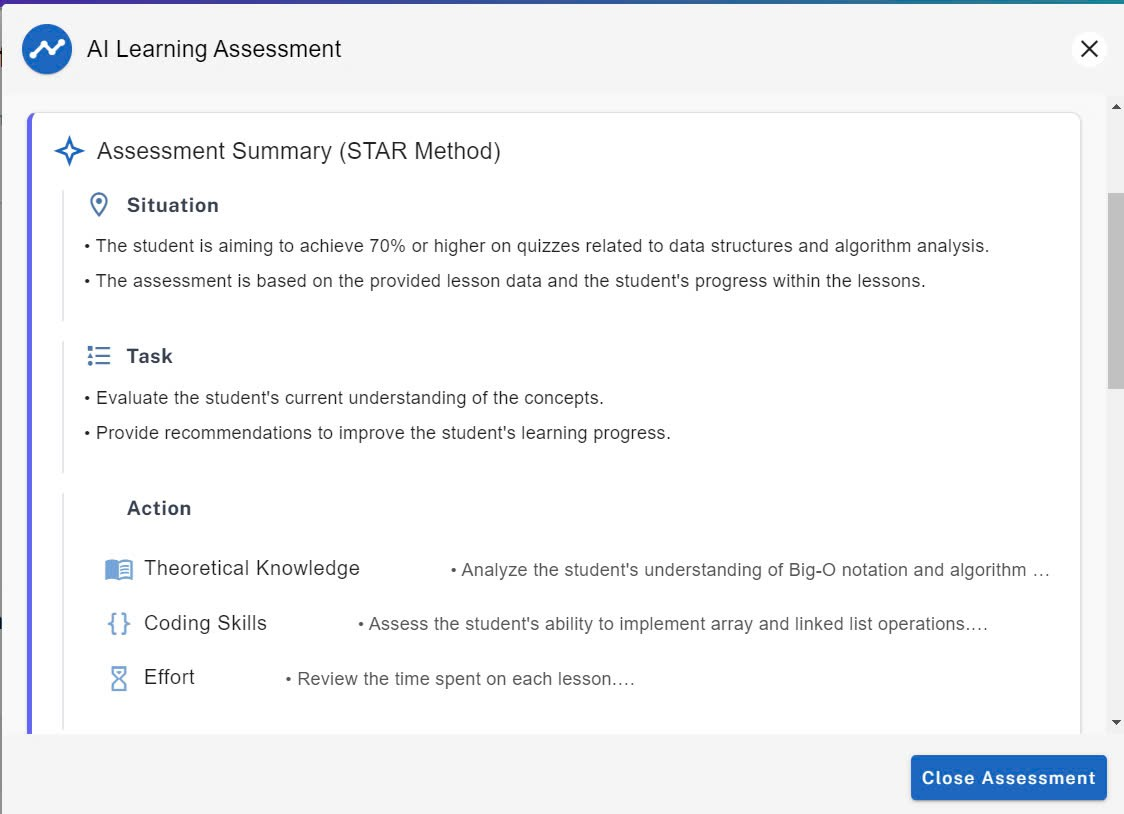
\includegraphics[width=0.8\textwidth]{Images/UI_LLM/Assessment_1.png}
\end{figure}
\begin{figure}[H]
    \centering
    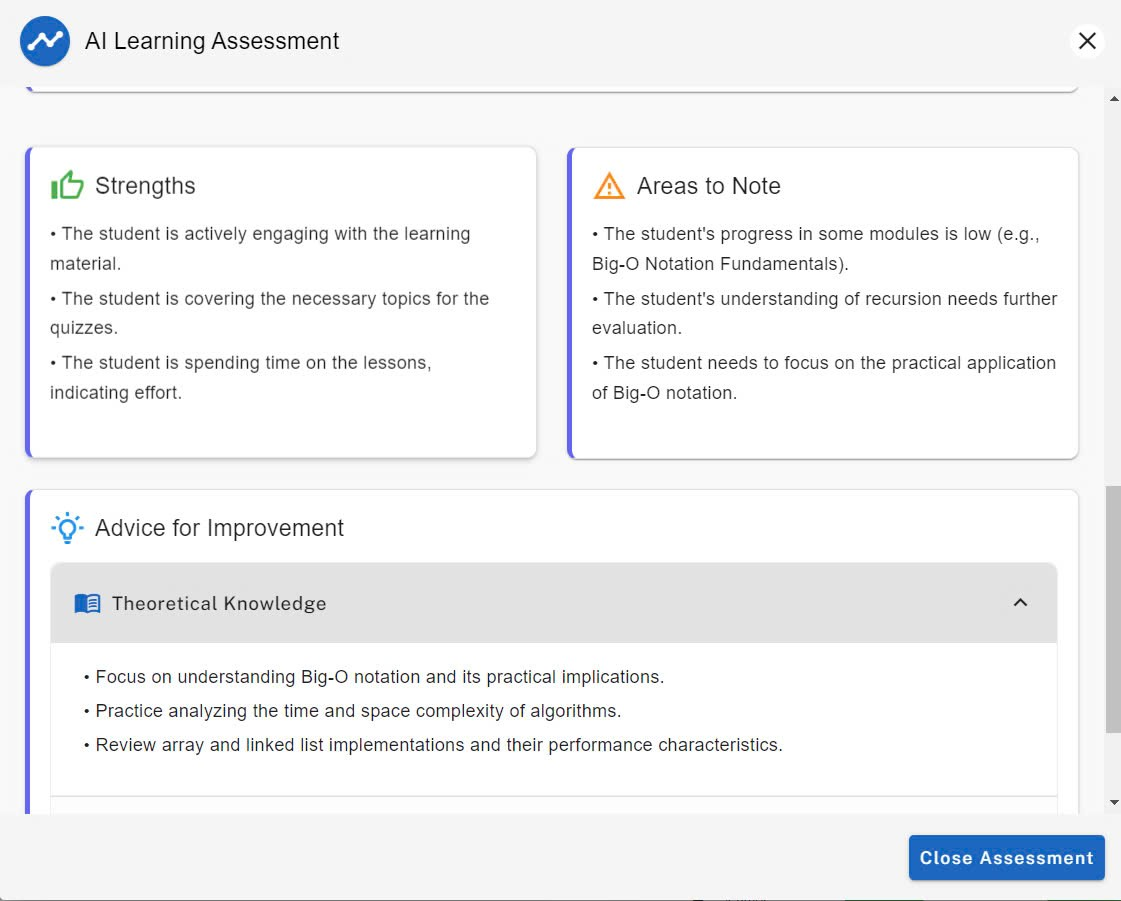
\includegraphics[width=0.8\textwidth]{Images/UI_LLM/Assessment_2.png}
    \caption{Báo cáo đánh giá học tập dựa trên phương pháp STAR}
\end{figure}
\subsection{Theo dõi và phân tích tiến độ học tập}
Hệ thống cung cấp API \texttt{/progress\_tracking/student/recommend\_lessons/\{recommend\_lesson\_id\}/time\_spent} để cập nhật thời gian học tập và theo dõi tiến độ của học sinh:

\begin{itemize}
    \item \textbf{Cập nhật thời gian}: Hàm \texttt{add\_time\_spent} nhận thời gian mới (định dạng HH:MM:SS) và cộng dồn vào thời gian hiện có.
    \begin{lstlisting}[language=Python]
def add_time_spent(existing_time_spent, new_time_spent_str):
    hours, minutes, seconds = map(int, new_time_spent_str.split(':'))
    new_time_delta = timedelta(hours=hours, minutes=minutes, seconds=seconds)
    return existing_time_spent + new_time_delta
    \end{lstlisting}
    \item \textbf{Lưu trữ}: Thời gian được cập nhật vào cơ sở dữ liệu qua \texttt{recommend\_lesson\_controller}.
    \item \textbf{Kết quả}: Trả về thời gian đã cập nhật, ví dụ:
    \begin{lstlisting}[language=JSON]
{
    "recommend_lesson_id": "xyz789",
    "updated_time_spent": "02:30:45"
}
\end{lstlisting}
\end{itemize}

Kết quả giao diện một báo cáo theo dõi tiến độ học tập, ví dụ:
\begin{figure}[H]
    \centering
    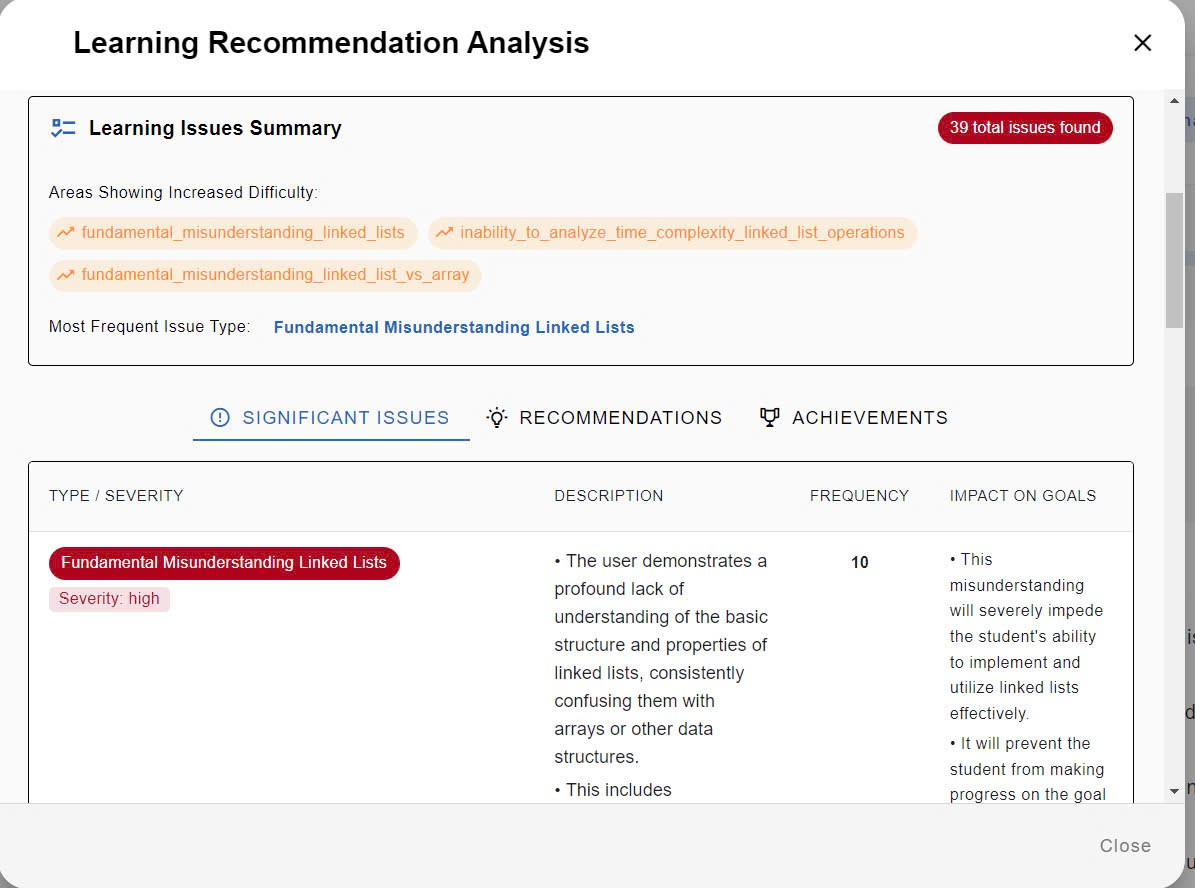
\includegraphics[width=0.8\textwidth]{Images/UI_LLM/tracking_issues.png}
    \caption{Báo cáo theo dõi những vấn đề trong quá trình học tập}
\end{figure}

\begin{figure}[H]
    \centering
    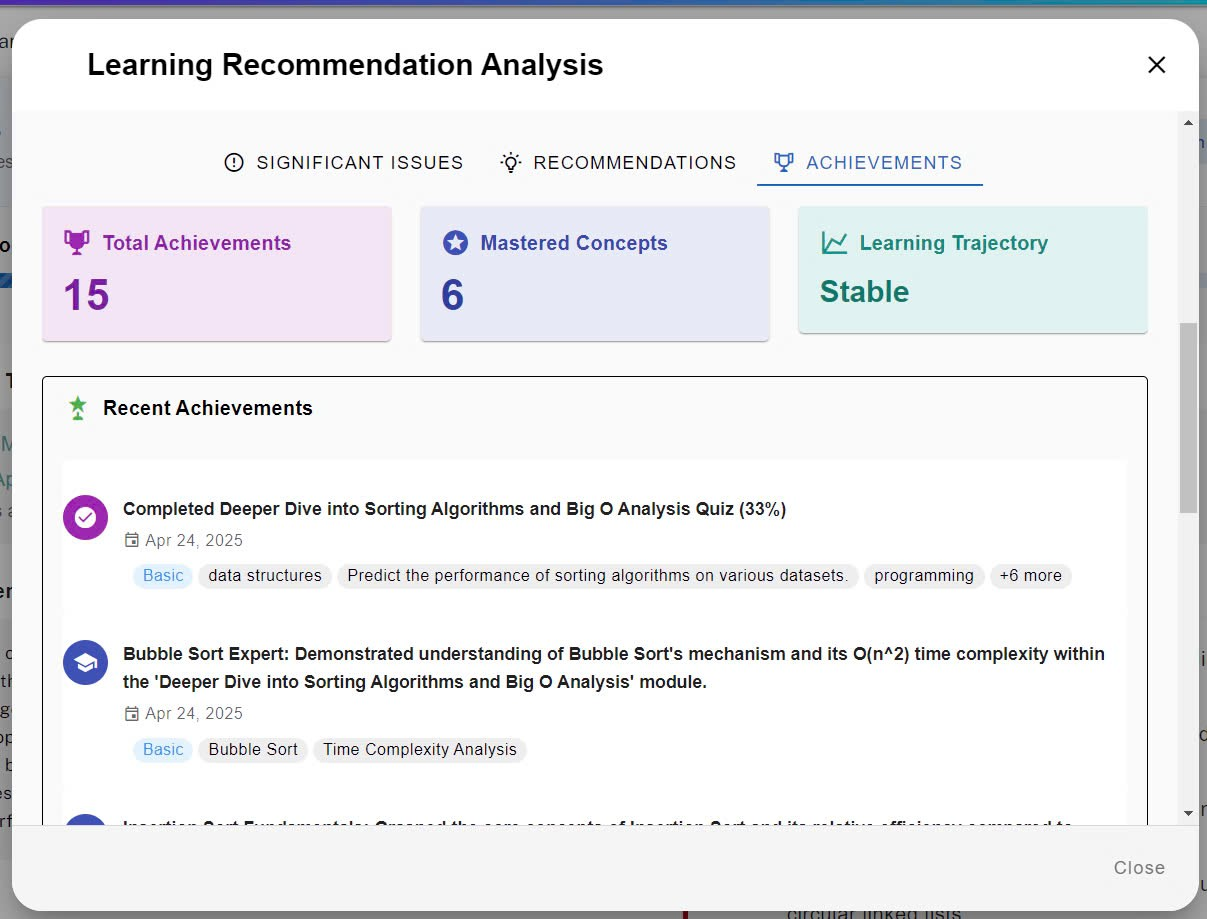
\includegraphics[width=0.8\textwidth]{Images/UI_LLM/tracking_achivement.png}
    \caption{Báo cáo theo dõi những thành tích trong quá trình học tập}
\end{figure}
\subsection{Đánh giá kết quả học tập (Monitor Study Progress)}
Phần này sử dụng API để phân tích kết quả sau khi học sinh hoàn thành một bài học được đề xuất. Các bước:
\begin{itemize}
    \item \textbf{Kiểm tra tiến độ}: Hệ thống kiểm tra xem học sinh đã đạt đủ tiến độ cần thiết (ít nhất 80\%) để được đánh giá.
    \item \textbf{Phân tích vấn đề}: Dựa trên \texttt{issues\_summary} từ cơ sở dữ liệu, hàm \texttt{analyze\_issues} sử dụng AI để xác định các vấn đề quan trọng (significant\_issues) và mức độ nghiêm trọng (severity).
    \item \textbf{Đề xuất hành động}: Đưa ra một hoặc hai khuyến nghị (proceed, repeat, review\_prior), ví dụ:
    \begin{lstlisting}[language=JSON]
{
    "can_proceed": false,
    "needs_repeat": true,
    "needs_review_prior": false,
    "issues_analysis": {
        "significant_issues": [
            {
                "type": "concept_misunderstanding",
                "frequency": 8,
                "description": "Struggling to grasp recursion base cases.",
                "severity": "high",
                "impact_on_goals": "This significantly hinders..."
            }
        ],
        "total_issues_count": 13,
        "increasing_issues": ["recursion application"],
        "most_frequent_type": "concept_misunderstanding"
    },
    "recommendations": [
        {
            "action": "repeat",
            "reason": "Significant difficulties with recursion...",
            "details": "Review 'Advanced Recursion'"
        }
    ]
}
    \end{lstlisting}
\end{itemize}

\section{Tạo bài kiểm tra (Generate Quiz)}
Chức năng này cho phép hệ thống tạo bài kiểm tra trắc nghiệm dựa trên nội dung của một module, sử dụng endpoint \texttt{/generate-quiz}. Các bước thực hiện:
\begin{itemize}
    \item \textbf{Tập hợp dữ liệu}: Hệ thống lấy thông tin từ module, bài học (lesson), nội dung được đề xuất (recommended content), và tài liệu liên quan (documents).
    \item \textbf{Tạo câu hỏi theo phân phối độ khó}: AI sinh ra các câu hỏi với ba mức độ khó (easy, medium, hard) theo phân phối được yêu cầu, sử dụng mô hình Gemini qua \texttt{AIToolProvider}. Ví dụ mã nguồn:
    \begin{lstlisting}[language=Python]
async def generate_quiz(request: GenerateQuizRequest, ...):
    # Fetch module details
    module = await modules_controller.modules_repository.first(
        where_=[Modules.id == request.module_id]
    )
    
    # Generate questions for each difficulty level
    for difficulty in difficulties:
        prompt = f"Generate EXACTLY {questions_needed} {difficulty_name} difficulty questions..."
        response = llm.invoke(question_request.content)
    \end{lstlisting}
    \item \textbf{Lưu trữ}: Câu hỏi và bài kiểm tra được lưu vào cơ sở dữ liệu với thông tin như thời gian giới hạn và điểm tối đa.
\end{itemize}
Kết quả là một JSON chứa bài kiểm tra, ví dụ:
\begin{lstlisting}[language=JSON]
{
    "quiz_id": "abc123",
    "name": "Quiz: Python Basics",
    "description": "Assessment covering key concepts from Introduction to Python",
    "time_limit": 30,
    "max_score": 100,
    "module_id": "def456",
    "questions": [
        {
            "id": "q123",
            "question_text": "What is a list in Python?",
            "question_type": "single_choice",
            "options": ["A mutable sequence type", "An immutable sequence type", "A mapping type", "A set type"],
            "correct_answer": ["A mutable sequence type"],
            "difficulty": "easy",
            "explanation": "Lists in Python are mutable sequences...",
            "points": 5
        }
    ]
}
\end{lstlisting}

Giao diện tạo một bài kiểm tra trắc nghiệm, ví dụ:
\begin{figure}[H]
    \centering
    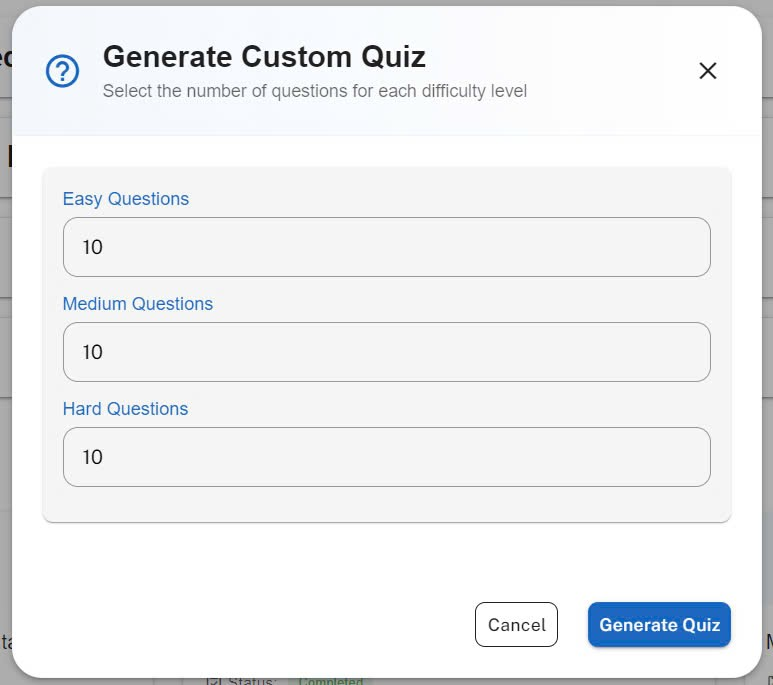
\includegraphics[width=0.5\textwidth]{Images/UI_LLM/Gen_quiz.png}
    \caption{Form tạo bài kiểm tra trắc nghiệm}
\end{figure}

Sinh viên có thể chọn độ khó của bài kiểm tra và số lượng câu hỏi cho mỗi độ khó. Sau khi tạo, bài kiểm tra sẽ được lưu vào cơ sở dữ liệu và có thể được truy cập từ giao diện người dùng.

\begin{figure}[H]
    \centering
    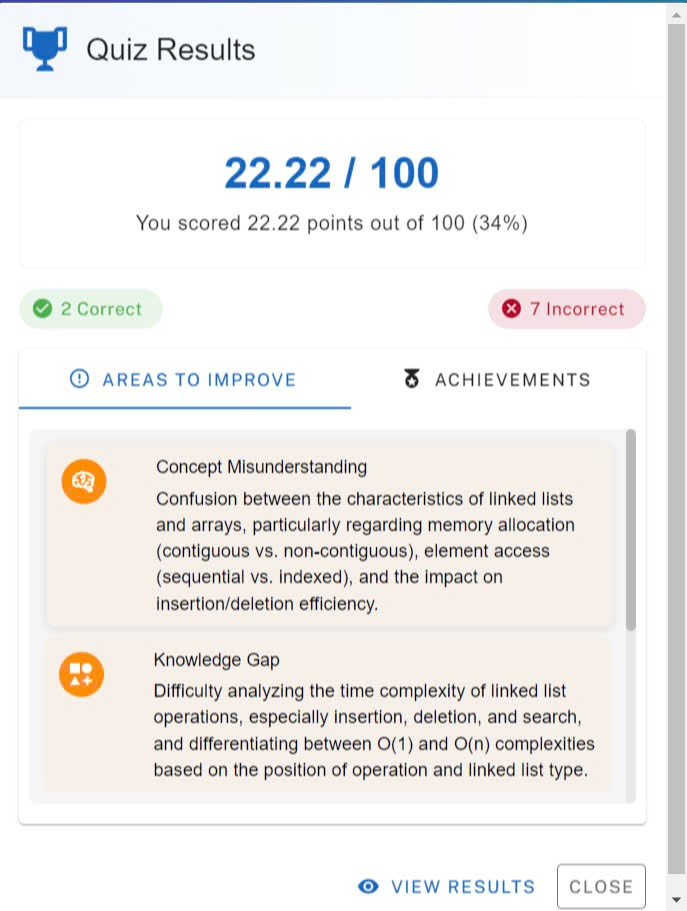
\includegraphics[width=0.6\textwidth]{Images/UI_LLM/Quiz_result.png}
    \caption{Kết quả bài kiểm tra trắc nghiệm}
\end{figure}

Sau khi hoàn thành một bài kiểm tra, sinh viên có thể xem kết quả và nhận phản hồi từ hệ thống. Hệ thống sẽ phân tích những vấn đề sinh viên gặp phải, những phần sinh viên nắm chắc và cung cấp các khuyến nghị cho sinh viên dựa trên hiệu suất của họ trong bài kiểm tra.
\section{Tạo bổ sung nội dung bài học (Regenerate Lesson Content)}
Chức năng này tạo thêm nội dung bài học bổ sung dựa trên các vấn đề học sinh gặp phải, sử dụng endpoint \texttt{/generate-supplemental-content}. Các bước:
\begin{itemize}
    \item \textbf{Phân tích vấn đề}: Dựa trên kết quả phân tích từ \texttt{monitor\_study\_progress}, hệ thống xác định các khía cạnh cần cải thiện (ví dụ: hiểu sai khái niệm, lỗi mã).
    \item \textbf{Đánh giá tình huống}: Kiểm tra mức độ khó khăn sinh viên đang gặp phải và xác định liệu vấn đề có cần tham chiếu đến kiến thức từ các bài học trước đó không (needs\_review\_prior). Hệ thống thu thập thông tin liên quan từ các bài học trước nếu cần thiết để cung cấp bối cảnh đầy đủ.
    \item \textbf{Tạo nội dung mới}: AI sinh nội dung cập nhật với các mô-đun chi tiết, ví dụ mã nguồn:
    \begin{lstlisting}[language=Python]
async def regenerate_lesson_content(
    recommend_lesson_id: UUID,
    analysis_result: dict,
    prior_recommend_lessons_data: List[dict],
    ...
):
    prompt = f"""
    ## Lesson Content Regeneration Task
    ### Context
    - Lesson Title: "{lesson.title}"
    - Analysis Result: {json.dumps(analysis_result, indent=2)}
    """
    updated_content = chunking_manager.call_llm_api(prompt, ...)
    \end{lstlisting}
    \item \textbf{Cập nhật dữ liệu}: Lưu các module bổ sung vào cơ sở dữ liệu và liên kết chúng với bài học hiện tại. Các module ban đầu vẫn được giữ nguyên, đảm bảo tính liên tục của lộ trình học tập.
\end{itemize}

Kết quả là một JSON chứa nội dung mới, ví dụ:
\begin{lstlisting}[language=JSON]
{
    "modules": [
        {
            "title": "Recursion Basics Revisited",
            "objectives": ["Understand base cases", "Apply recursive patterns"],
            "reading_material": {...}
        }
    ]
}
\end{lstlisting}
Nội dung bổ sung được thiết kế để giải quyết các vấn đề cụ thể mà sinh viên đang gặp phải, đồng thời duy trì tính liên tục của lộ trình học tập. Các module bổ sung này tập trung vào việc làm rõ những khái niệm khó, cung cấp thêm ví dụ minh họa, và tạo cơ hội thực hành có hướng dẫn. Cách tiếp cận này giúp sinh viên vượt qua những khó khăn cụ thể mà không cần phải học lại toàn bộ nội dung
\section{Kiến trúc tổng thể hệ thống}
Hệ thống học tập trực tuyến thông minh được thiết kế theo mô hình Client – Server, với các thành phần chính bao gồm:

\subsection{Frontend (Client-side):}
Được xây dựng bằng Vue 3, giao diện người dùng cung cấp các tính năng như đăng nhập, học bài, làm bài tập, theo dõi tiến độ học tập, tương tác với gia sư AI, gửi phản hồi, \dots

Frontend giao tiếp với backend thông qua các API RESTful.

\subsection{Backend (Server-side):}
Đảm nhiệm xử lý logic nghiệp vụ, quản lý dữ liệu người dùng, khóa học, bài học, bài tập, tiến độ học, phản hồi, \dots Đồng thời xử lý yêu cầu từ AI (qua LLM API).
Backend được xây dựng bằng FastAPI. 
\subsection{Cơ sở dữ liệu (Database):}
Sử dụng hệ quản trị cơ sở dữ liệu PostgreSQL để lưu trữ thông tin người dùng, khóa học, bài học, kết quả học tập, bài tập, phản hồi, \dots
Thiết kế cơ sở dữ liệu đảm bảo tính mở rộng, hỗ trợ việc theo dõi tiến độ và sinh báo cáo.

\subsection{AI Module (LLM – Large Language Model):}
Các tác vụ như gợi ý lộ trình học, sinh bài tập, chấm điểm và hỗ trợ giải thích được thực hiện nhờ tích hợp LLM API (OpenAI, Gemini)
Backend sẽ định nghĩa prompt phù hợp và gửi yêu cầu tới LLM để lấy kết quả.

\subsection{Hệ thống lưu trữ tài liệu:}
Các tài liệu PDF, slide bài giảng được lưu ở AWS S3 thư mục local server.

\section{Sơ đồ cơ sở dữ liệu}
\begin{figure}[H]
    \centering
    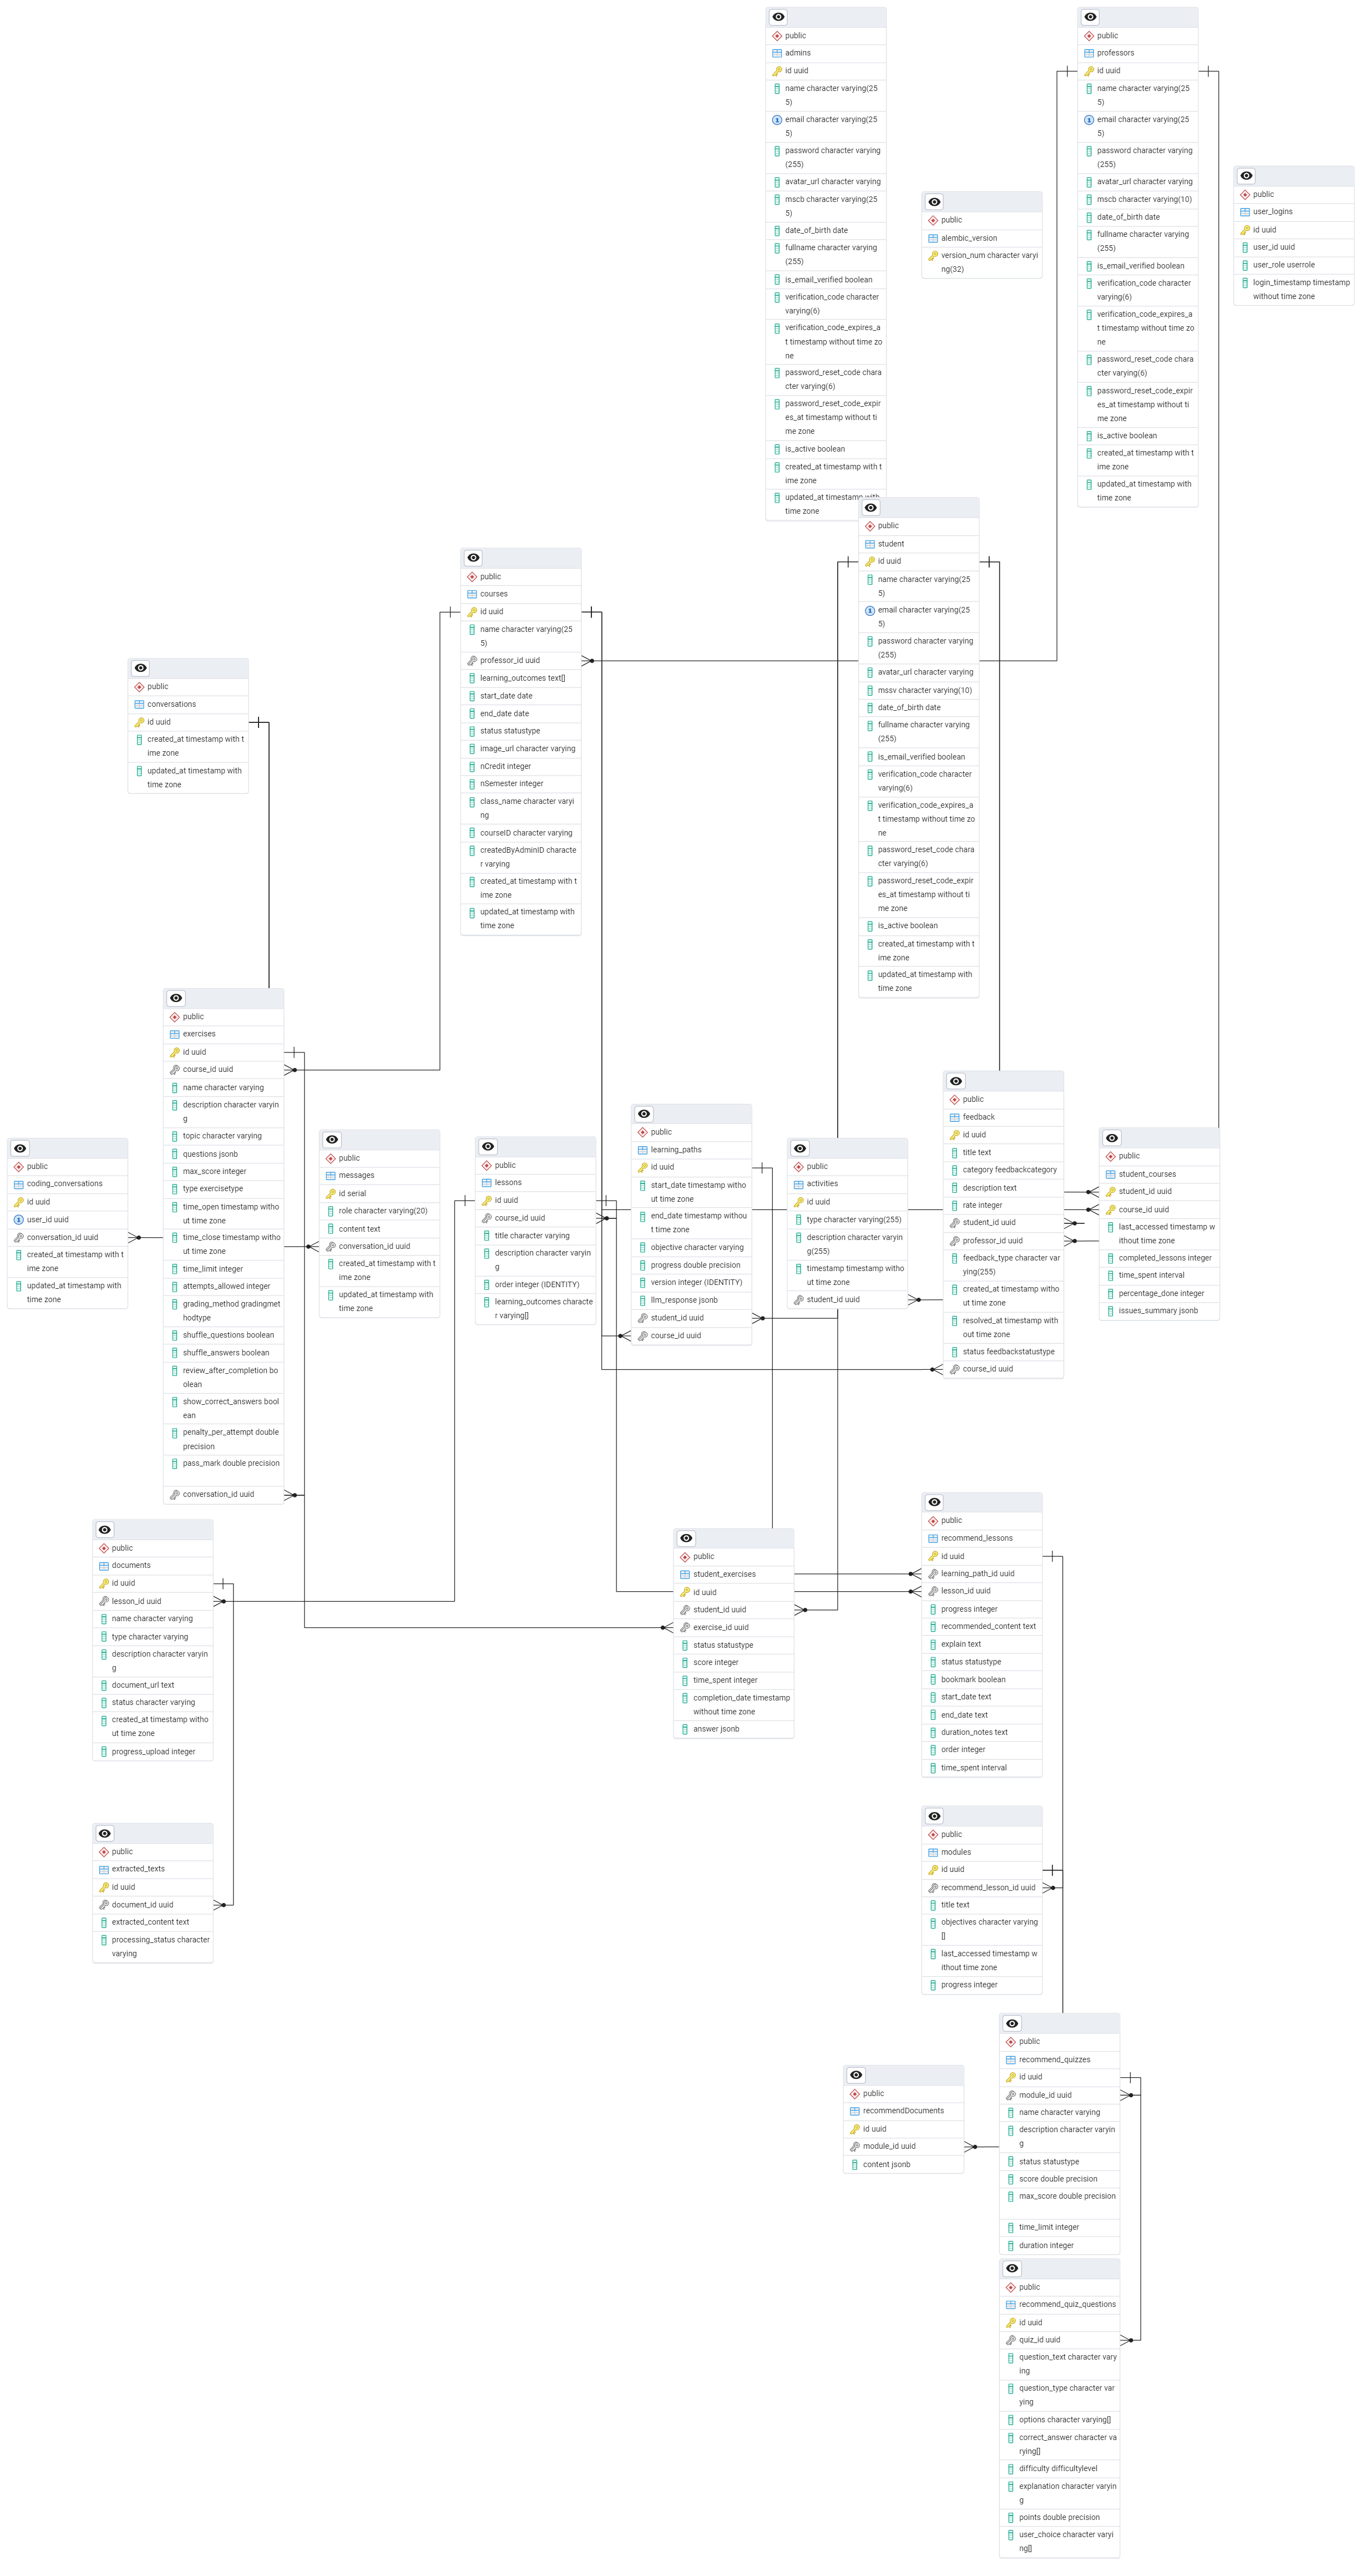
\includegraphics[width=0.6\linewidth]{images/ERD.png}
    \caption{Sơ đồ cơ sở dữ liệu của hệ thống}
    \label{fig:enter-label}
\end{figure}

\subsection{Tổng quan cấu trúc cơ sở dữ liệu}
Hệ thống được xây dựng trên nhiều bảng chính, chia thành các nhóm chức năng như sau:

\subsubsection{Nhóm người dùng (User Management)}
\begin{itemize}
    \item \textbf{professors}, \textbf{student}, \textbf{admins}: chứa thông tin cơ bản của người dùng theo 3 role như username, email, password,...
    \item \textbf{user\_login}\: bảng mở rộng lưu thông tin đăng nhập người dùng.
\end{itemize}

\subsubsection{Nhóm khóa học và tài liệu (Course Management)}
\begin{itemize}
    \item \textbf{courses}, \textbf{student\_courses}, \textbf{extracted\_text}: quản lý thông tin khóa học, tham gia khóa học và tài liệu học tập liên quan do giảng viên đăng tải.
    \item \textbf{lessons}, \textbf{documents}, \textbf{modules}: quản lý bài học và các nội dung bài học liên quan.
    \item \textbf{learning\_paths}, \textbf{recommend\_lessons}, \textbf{recommend\_documents}: quản lý các bài kiểm tra, bài tập và câu hỏi liên quan đến khóa học.
\end{itemize}

\subsubsection{Nhóm câu hỏi và bài kiểm tra (Assessment)}
\begin{itemize}
    \item \textbf{recommend\_quizzes}, \textbf{exercises}: chứa thông tin về các câu hỏi, loại câu hỏi, câu trả lời và kết quả bài kiểm tra của sinh viên trong các bài quiz được sinh ra theo từng bài học đề xuất.
\end{itemize}

\subsubsection{Nhóm tương tác và phản hồi (Interaction)}
\begin{itemize}
    \item  \textbf{feedbacks}, \textbf{activities}: quản lý tương tác giữa sinh viên và giảng viên, người dùng và hệ thống, và các hoạt động của người dùng.
\end{itemize}

\subsubsection{Nhóm bài tập Code Exercises}
\begin{itemize}
    \item \textbf{conversations}, \textbf{messages}, \textbf{coding\_conversations}: ghi nhận nhật ký hoạt động, cài đặt hệ thống và quản lý phiên làm việc.
\end{itemize}

\subsection{Mối quan hệ giữa các bảng}
Các bảng trong hệ thống có mối quan hệ nhiều-nhiều và một-nhiều, với các khóa ngoại được thể hiện rõ trong sơ đồ:
\begin{itemize}
    \item Một người dùng có thể tham gia nhiều khóa học thông qua bảng \texttt{student\_courses}.
    \item Một khóa học có thể có nhiều bài học, bài kiểm tra và tài liệu.
    \item Bài kiểm tra có thể bao gồm nhiều câu hỏi và mỗi câu hỏi có nhiều đáp án.
    \item Người dùng có thể đưa ra phản hồi và nhận thông báo từ hệ thống.
    \item Một sinh viên đối với một khóa học có thể có nhiều lộ trình học khác nhau. 
    \item Một lộ trình học có thể có nhiều bài học và tài liệu khác nhau.
    \item Một bài học có thể có nhiều module nhỏ và nội dung khác nhau.
    \item Một module có thể có nhiều bài quiz hoặc code exercises khác nhau (do sinh viên tùy chọn sinh ra)
\end{itemize}

\subsection{Kết luận}
Sơ đồ ERD này cung cấp một cái nhìn toàn diện về kiến trúc cơ sở dữ liệu của hệ thống. Cấu trúc được tổ chức hợp lý, cho phép dễ dàng mở rộng và tích hợp thêm các chức năng mới như AI hỗ trợ học tập, phân tích dữ liệu học viên, và hơn thế nữa.

\section{Kết luận}
Hệ thống học tập trực tuyến thông minh đã được phát triển với mục tiêu mang lại trải nghiệm học tập cá nhân hóa, hiệu quả và linh hoạt cho sinh viên ngành công nghệ thông tin và những người có nhu cầu học lập trình. Thông qua việc tích hợp các mô hình ngôn ngữ lớn (LLM) và các tính năng tiên tiến như gia sư AI, hệ thống tạo bài tập tự động, và lộ trình học tập cá nhân hóa, hệ thống không chỉ hỗ trợ người học trong việc tiếp thu kiến thức mà còn giúp họ phát triển kỹ năng lập trình một cách thực tế và sâu sắc.

Các module đã được triển khai, bao gồm quản lý tài khoản, khóa học, bài học, bài tập, lộ trình học tập, tiến độ học tập, phản hồi, người dùng, nhật ký đăng nhập và dashboard, đáp ứng đầy đủ các yêu cầu chức năng và phi chức năng được đề ra. Những tính năng này cho phép sinh viên, giảng viên và quản trị viên tương tác một cách hiệu quả, đồng thời đảm bảo tính bảo mật, khả năng mở rộng và hiệu năng cao của hệ thống.

Trong tương lai, hệ thống có thể được cải tiến thêm bằng cách tích hợp các công nghệ mới, mở rộng các tính năng hỗ trợ đa ngôn ngữ, hoặc tối ưu hóa thuật toán đề xuất để nâng cao độ chính xác và phù hợp của các tài nguyên học tập. Với nền tảng vững chắc đã được xây dựng, hệ thống hứa hẹn sẽ tiếp tục là một công cụ hữu ích, đóng góp tích cực vào quá trình học tập và giảng dạy trong lĩnh vực công nghệ thông tin.
